%\documentclass[paper]{geophysics}
\documentclass[manuscript,revised]{geophysics}
\usepackage{amsmath}
\usepackage{xcolor}
%\usepackage{xcolor}
%\usepackage{graphicx}
%\usepackage[printfigures]{figcaps}
%\usepackage{float}
%\usepackage[caption = true]{subfig}
\PassOptionsToPackage{caption = true, position=top}{subfig}
\captionsetup[subfigure]{position=top,textfont=normalfont,singlelinecheck=off,justification=raggedright}


\newcommand{\sendatend}[1]{\AtEndDocument{#1 \clearpage}}
%\newcommand{\sendatend}[1]{#1}

\newcommand\norm[1]{\left\lVert#1\right\rVert}

\graphicspath{ {../figures/} }

\begin{document}

\title{Shape-constrained Geophysical Inversion}

\renewcommand{\thefootnote}{\fnsymbol{footnote}} 
%\ms{} % paper number
%\footer{Test}
\lefthead{Denli \& Brandman}
\righthead{Shape-Constrained Geophysical Inversion}

\address{
\footnotemark[1] ExxonMobil Research \& Engineering Company, \\
1545 Route 22E, Annandale, NJ 08801}
\author{Huseyin Denli\footnotemark[1] and Jeremy S. Brandman\footnotemark[1]}

\maketitle

\begin{abstract}
Two long-standing challenges for geophysical inverse problems are non-uniqueness (especially in the multi-parameter setting) and the slow convergence of gradient-based optimization methods.  This paper introduces shape-based inversion algorithms to address these challenges.  The shape-based algorithms presented here determine, based on the available geophysical data, both the underlying subsurface structures (e.g. stratigraphic layers) and the spatially varying unknown physical parameters (e.g. velocity and density).  Inverting simultaneously for geologic structures and physical parameters eliminates degeneracies between parameters and also provides a multi-scale framework for decomposing the inverse problem.  The first part of this paper provides a rigorous mathematical formulation of shape-based algorithms through diffuse interface approximations.  The second part demonstrates the applicability of these algorithms to a range of synthetic model problems in travel time tomography, full-waveform inversion, gradiometry, and history matching of single-phase flow.  These examples highlight the ability of shape-based inversion to mitigate non-uniqueness and improve the rate of convergence to a physically realistic solution.    
\end{abstract}

\section{Introduction}
Geophysical inversion determines the value of one or more geophysical parameters of a subsurface region (e.g., wave speeds/velocities, anisotropy parameters, clay volume fraction, porosity, electrical conductivity, and density) in a manner which is consistent with the available geophysical data (e.g., seismic, time-lapse seismic, electromagnetic, gravity, gradiometry, well log, and well pressure measurements)  acquired at locations remote from the region.  It is often carried out through the minimization of an objective function which includes a least-squares data misfit and a regularization term~\cite[]{Parker_1994}. Such an objective function typically takes the form
\begin{equation} \label{eq:objective}
J\left(\kappa\right) = \int_M \norm{u(\kappa)-\bar{u}}^2  dx + R\left(\kappa\right),
\end{equation}
where $\kappa$ represents the unknowns to be determined through optimization, $\bar{u}$ is the measured geophysical data, $u(\kappa)$ is data computed according to a mathematical model, $M$ denotes the locations at which the data is measured,$\norm{}$ is an arbitrary norm used to quantify the error or misfit between the computed data $u(\kappa)$ and the measured data $\bar{u}$, and $R\left(\kappa\right)$ is a regularization term (e.g. Tikhonov regularization ) used to stabilize the inversion. 

The unknown $\kappa$ is typically discretized, for computational purposes, when optimizing the objective function $J\left(\kappa\right)$. Such a discretization amounts to first partitioning the subsurface domain $\Omega$ into disjoint cells $\Omega_i$, such that $\Omega = \cup\Omega_i$, and then setting $\kappa(x)=\kappa_i$ for $x \in \Omega_i$.  One example of such a partitioning into cells is a regular Cartesian grid. The parameter values ${\kappa_i}$ are then typically determined by optimizing equation~\ref{eq:objective} using a gradient-based optimization technique such as Gauss-Newton, quasi-Newton, or steepest descent. Henceforth, this approach will be referred to as cell-based inversion~\cite[]{Aster_2013}.

Many geophysical inverse problems, especially multi-parameter problems (e.g. full-wavefield inversion of density and wave speed), are under-constrained or sensitive to noise in the available data.  For such problems, cell-based inversion does not yield satisfactory results.  Regularization is often included in equation \ref{eq:objective} in order to address these issues, but state-of-the-art regularization methods may introduce artifacts (e.g. unnecessary smoothing); further, such regularization may not fully eliminate the non-uniqueness present.  

In this paper, we introduce geophysical inversion techniques that mitigate non-uniqueness by constraining the unknown physical parameters to be structurally consistent.  Structural consistency of two parameters means that the parameters share a common set of interfaces across which the parameters' profiles  change abruptly.  Since many geologic parameters exhibit such a relationship (e.g. wave speed and density), structural consistency is a natural constraint to impose on multi-parameter inverse problems.  

Three distinct approaches to enforcing structural consistency were proposed previously.  The first links the different unknown parameters through geophysical or empirical relationships (e.g., Archie’s law) and inverts for a minimal subset of the parameters. When well-known relationships between parameters are available, this approach has great appeal. However, such relationships are, in many cases, either poorly understood or unknown completely, rendering this approach of limited value.  The second approach, known as the cross-gradient approach, inverts for two distinct physical parameters by introducing an additional term into the objective function which penalizes gradients that are not collinear \cite[]{Haber_1997,Gallardo_2007}. As a result, this approach encourages structural consistency, but it does not strictly enforce it. In addition, it is unclear how this approach generalizes to an arbitrary number of different physical parameters. 
A third strategy uses level-set functions to represent interfaces between subsurface regions~\cite[]{Kadu_2016}. This approach has been applied to inverse problems such as full-wavefield inversion, gravity inversion~\cite[]{Li_2016}, magnetic inversion~\cite[]{Li_2017}, and reservoir history matching. However, due to the nature of the level-set representation, it is unclear how effective this approach will be for problems with either a large number of distinct subsurface regions or regions with significant heterogeneity. 

\section{Methodology}

\subsection{Overview}
In this paper, we propose flexible shape-based inversion algorithms that ensure structural consistency while inverting for interfaces and the associated subsurface parameter values.  Before going into the details of the algorithms, we first define a number of terms that are used throughout the paper.  First, the terms \textbf{shape, geologic structure,} and \textbf{geobody} will be interchangeably used to refer to a three dimensional portion of the subsurface which is part of a single facies or part of a single stratigraphic layer.  Examples of such features include, but are not limited to, salt bodies, shale layers, sandstone formations, carbonate platforms, and hydrocarbon reservoirs.  Second, the term \textbf{interface} refers to those subsurface locations at the boundary between two shapes.  For example, there exists an interface separating different sedimentary layers.  At an interface between shapes, we expect that the profile of at least one of the geophysical parameters will change in an abrupt or discontinuous matter.  Third, the term \textbf{geologic feature} is used to refer to either a shape or an interface.  Fourth, the term \textbf{structurally consistent inversion} refers to an inversion of multiple geophysical parameters (e.g. wave speed and density) in which the different parameter types possess a common set of shapes along with a common set of interfaces at which parameter values may change sharply or discontinuously. 

Underpinning this work is the belief that a structurally consistent inversion, consisting of the inversion of geologic features and the underlying geophysical parameters, will yield a result of greater fidelity than an inversion of geophysical parameters alone.  We also believe that shape-based inversion provides other benefits over cell-based approaches.  First, shape-based inversion has the potential to reduce the number of degrees of freedom and improve convergence properties.  This may be accomplished by assigning constant parameter values within each geobody.   Second, geologic features are often of intrinsic value; automatic identification eliminates manual picking of subsurface structures or the application of additional algorithms to do so.

The algorithms presented below are based on implicit shape representations of geologic features.  Implicit representations are those in which shapes are described implicitly through the use of one or more auxiliary functions defined on a predetermined cellular grid (e.g. a Cartesian grid). Unlike explicit shape representation methods~\cite[]{Galley20}, implicit methods are desirable because they naturally handle merging and breaking of shapes, as well as regions of high curvature, without any change in algorithm, discretization, or grid.   In contrast, it is nontrivial to ensure that explicit techniques accommodate topological changes and such algorithms can also exhibit numerical instabilities near regions with high curvature~\cite[]{Abubakar_2009}.  For further discussion of implicit and explicit methods, see~\cite{Osher_1988}.

We present two inversion techniques for the identification of geologic features and subsurface parameter values.  The first, referred to as Mumford-Shah inversion, simultaneously inverts for interfaces and geophysical parameters $\kappa$. The second, referred to as phase-field inversion, inverts for geologic shapes and a parameter field $\kappa$ obeying a pre-determined trend (e.g., piecewise constant or piecewise linear). Mumford-Shah inversion is more general in that it can capture an arbitrary number of interfaces along with heterogeneous $\kappa$ fields. In contrast, phase-field inversion requires the user to specify the maximum number of shapes in advance, along with expected trend behavior (e.g. linear or quadratic) of each parameter.  Which method is appropriate for a given problem depends on what is known in advance regarding the geophysical parameters of interest and the information content of the measured data. 

\subsection{Mumford-Shah}
\subsubsection{Continuous Formulation}
Our first approach to shape-based inversion utilizes the Mumford-Shah functional, introduced for image segmentation by~\cite{Mumford_1989}.  In order to invert for geophysical parameter values $\kappa$ in a structurally consistent manner, the Mumford-Shah-based inversion technique decomposes the subsurface region of interest into distinct shapes separated by interfaces. These interfaces, along with the values of the parameter $\kappa$ within each of the shapes, may be determined by optimizing an objective function $E$. The objective function $E$ is
\begin{equation} \label{eq:shape}
E\left(\kappa,\Gamma\right)=\int_M \norm{u(\kappa)-\bar{u}}^2  dx+MS\left(\kappa,\Gamma\right),	
\end{equation}
where $\kappa$ and $\Gamma$ are the unknowns to be determined through the optimization, with $\kappa$ being values of the subsurface parameters and $\Gamma$ consisting of the set of interfaces separating the shapes. $\bar{u}$ is the measured geophysical data and $u(\kappa)$ is data computed by a forward model during the optimization of the objective function $E$. The operator $\norm{}$  is an arbitrary norm used to quantify the error or misfit between the computed data and the measured data. $M$ is a domain describing spatial locations of the measured geophysical data $\bar{u}$. 

The objective function in equation \ref{eq:shape} can be broken down into two contributions.  The first term is the data misfit  $\int_M \norm{u(\kappa)-\bar{u}}^2  dx$, which ensures that the inferred parameter values $\kappa$ are consistent with the measured geophysical data $\bar{u}$.  The second term is the function $MS$, known as the Mumford-Shah functional~\cite[]{Mumford_1989}. The Mumford-Shah functional $MS$ partitions the subsurface region of interest into shapes, enforces some degree of homogeneity (i.e., smoothness) of $\kappa$ within each shape, and controls the complexity of the interface set $\Gamma$. 

The Mumford-Shah functional $MS$ is given by
\begin{equation} \label{eq:MS}
MS(\kappa,\Gamma)=\alpha \int_{\Omega\backslash\Gamma} F(\kappa) dx + \beta\int_\Gamma \norm{t(s)}_\Gamma  ds ,
\end{equation}
where the spatial domain $\Omega$ represents the subsurface region of interest.  The function $F$ appearing in the first integrand is a regularization function ensuring that the values of $\kappa$ vary smoothly within each shape; the most common choice is $F(\kappa)=\left\vert \nabla \kappa \right\vert^2$.   The second integrand in equation \ref{eq:MS} measures arclength and penalizes oscillations of the interface set $\Gamma$ within each of the subsurface shapes.  Here, $t(s)$ is a tangent vector of the interface $\Gamma$, and the operator $\norm{}_\Gamma$ is an arbitrary norm, potentially anisotropic, used to measure arclength.  Lastly, the weights $\alpha$ and $\beta$ control the magnitude of the contributions of the two terms described above.  

%\begin{equation} \label{eq:Tikhonov}
%(\kappa)=\left\vert \nabla \kappa \right\vert^2
%\end{equation}

We close this section by highlighting two useful properties of the Mumford-Shah functional.  First, it is capable of partitioning a subsurface region into an arbitrary number of shapes and interfaces. Second, it permits a wide range of spatial variation in the geophysical parameters $\kappa$ within each shape.

\subsubsection{Discretization}
The search for a minimizing pair $(\kappa,\Gamma)$ of the objective function $E$ in equation \ref{eq:shape} is generally non-trivial due to the potential complexity of the interface set $\Gamma$.  Throughout this paper, we assume that arclength is measured using the Euclidean norm; this allows us to use the Ambrosio-Tortorelli approximation $MS_\epsilon$ \cite[]{Ambrosio_1992} of the Mumford-Shah functional given in equation \ref{eq:MS}.  The Ambrosio-Tortorelli approximation is given by %equation~\ref{eq:epsilon}.
\begin{equation} \label{eq:epsilon}
MS_\epsilon (\kappa,\phi)=\alpha \int_\Omega \phi^2 F(\kappa) dx + \beta \int_\Omega  \left( \epsilon \left\vert \nabla \phi \right\vert^2+\frac{(\phi-1)^2}{4\epsilon} \right)   dx.	
\end{equation}
The Ambrosio-Tortorelli approximation $MS_\epsilon$ replaces the minimizing pair $(\kappa,\Gamma)$ by a minimizing pair $(\kappa_\epsilon,\phi_\epsilon)$.  It can be shown that, for $\epsilon \ll 1$,  $ MS_\epsilon (\kappa_\epsilon,\phi_\epsilon ) \approx MS(\kappa,\Gamma)$, $\kappa_\epsilon \approx \kappa$, and $\phi_\epsilon \approx 1$ except in a boundary layer of thickness O($\epsilon$)  near the boundary set $\Gamma$, where $\phi_\epsilon \approx 0$.  Hence, the location of $\Gamma$ may be approximated from knowledge of $\phi_\epsilon$.  

Minimization of the Ambrosio-Tortorelli approximation in equation \ref{eq:epsilon} requires a discretization of the variables $\kappa$ and $\phi$, along with discrete integration and differentiation operators.  In addition, the mesh size $h$ of the underlying grid must satisfy $h\ll\epsilon$ in order to resolve the boundary layer of $\phi_\epsilon$ near the interface set $\Gamma$ and ensure convergence.  Given such a discretization of the variables $\kappa$ and $\phi$, optimization may be performed using a gradient-based optimization method such as Gauss-Newton, quasi-Newton, or steepest descent.  The interface set $\Gamma$ is determined from the cell values of $\phi_\epsilon$.

\begin{comment}
The optimization procedure described above amounts to the determination of cell-based values of $\kappa$ and $\phi$ which minimize the objective function~\ref{eq:shape} using the approximation~\ref{eq:epsilon}.  On a formal level, this procedure resembles the traditional cell-based inversion approach.  However, the results of the Mumford-Shah and cell-based inversion strategies can differ significantly due to differences in the objective functions for these two techniques.  This difference is due to the regularization technique used by each method.  For example, cell-based inversion using first-order Tikhonov regularization (i.e. $R(\kappa)=\int_\Omega \left\vert \nabla \kappa \right\vert^2  dx$) leads to parameter values $\kappa$ which are uniformly smooth.  In contrast, Mumford-Shah inversion based on equations \ref{eq:shape}, \ref{eq:Tikhonov}, and \ref{eq:epsilon} enforces smoothness of $\kappa$ only within individual shapes.  
\end{comment}

\begin{comment}
    Another approach to approximating the Mumford-Shah functional MS is the Chan-Vese level-set approach~\cite[]{Chan_2001}. While the Ambrosio-Tortorelli approximation minimizes a functional $MS_\epsilon$ approximating the original Mumford-Shah functional $MS$, the Chan-Vese level-set approach instead directly optimizes for the interface set $\Gamma$ along with a constant parameter value associated with each shape determined by $\Gamma$. The Chan-Vese approach carries out this optimization by representing interfaces and shapes with a vector level-set function, which is then optimized along with piecewise constant parameter values for each shape. 
\end{comment}


\subsection{Phase-field}
\subsubsection{Continuous Formulation}

For problems in which the number of shapes and the expected trend of the parameters $\kappa$ (e.g piecewise constant or linear) are known in advance, an alternative inversion method known as the phase-field inversion technique may be advantageous. In contrast with the Mumford-Shah-based inversion technique, the phase-field inversion technique prescribes at the outset the maximum number of shapes to be inverted as well as information regarding the trend of the parameters $\kappa$ within each shapes (e.g., restricting the parameters $\kappa$ to be constant in each). 

Phase-field inversion can be seen as a technique for approximately decomposing a spatial domain $\Omega$ into disjoint shapes $\Omega_i$.  In the context of geophysical inversion, the decomposition of $\Omega$ into disjoint shapes $\Omega_i$, along with corresponding parameter values $\kappa_i$, arises from optimizing the objective function $H$
\begin{equation} \label{eq:pf}
H \left( \kappa_1,…,\kappa_n, \Omega_1,…,\Omega_n \right) = \int_M \norm{u(\kappa)-\bar{u}}^2 dx+ \beta \sum_{i=1}^n \int_{\partial\Omega_i \cap \Omega} \norm{t(s)}_{\partial\Omega_i} ds ,
\end{equation}
where $\bar{u}$ is the measured geophysical data and $u(\kappa)$ is data computed from a forward model.  Similar to Mumford-Shah, the operator $\norm{}$ is an arbitrary norm used to quantify the data misfit, M is a domain describing spatial locations of the measured geophysical data, $t(s)$ represents a tangent vector at the interface $\partial\Omega_i$ and $\norm{}_{\partial\Omega}$  is an arbitrary norm measuring arclength. A spatially-varying parameter field may be defined by $\kappa(x)=\kappa_i (x)$ for $x \in \Omega_i$.  

The objective function $H$ can be decomposed into a data misfit contribution and an interface penalization. The data misfit $\int_M \norm{u(\kappa)-\bar{u}}^2  dx$
%$\int_M \norm{u(\kappa)-\bar{u}}^2  dx$ 
ensures that the inferred parameter values $\kappa_i$ are consistent with the measured geophysical data $\bar{u}$. The interface penalization 
$\beta \sum_{i=1}^n \int_{\partial\Omega_i \cap \Omega} \norm{t(s)}_{\partial\Omega}  ds$
ensures that the interfaces of the shapes $\Omega_i$ do not exhibit unphysical oscillations. The constant $\beta$ controls the complexity of the shapes $\Omega_i$.
\begin{comment}
    There are two methods that are commonly used to optimize the objective function $H$ -- the phase-field approximation and the level-set method.  The phase-field technique has traditionally been used in materials science and physics to describe phase transitions and other interfacial phenomena~\cite[]{Chen_2002}.  The phase-field method~\cite[]{Deckelnick_2005} represents and moves shapes using a function which is equal, approximately, to one inside of the shape and equal, approximately, to negative one outside of the shape.  In addition, there is a narrow transition layer where the function transitions between the values of one and negative one.  Because the phase field technique does not explicitly identify the boundary of the shape, it is known as a diffuse interface method.   
\end{comment}

Phase-field provides a means of approximating equation~\ref{eq:pf} using an order parameter $\phi$.  For simplicity, assume that the number of shapes to be determined in equation~\ref{eq:pf} is restricted to two (i.e., $\Omega_2=\Omega\backslash\Omega_1$), measure arclength using the Euclidean norm, and assume that the subsurface model is piecewise constant.  In this context, the phase-field inversion amounts to the determination of a phase-field function $\phi_\epsilon:\Omega \rightarrow R$ and parameter values $\{ \kappa_{(\epsilon,1)}, \kappa_{(\epsilon,2)} \}$ minimizing the objective function 

\begin{equation} \label{eq:pf_epsilon}
H_\epsilon \left( \kappa_1,\kappa_2,\phi \right)=\int_M \norm{u(\kappa)-\bar{u}}^2  dx +\frac{\beta}{2} \left( \epsilon \int_\Omega \left\vert \nabla \phi \right\vert^2 dx+\frac{1}{\epsilon} \int_\Omega  \left( \phi^2-1 \right)^2 dx \right)
\end{equation}
for $\epsilon \ll 1$.  For reasons to be explained below, we define the parameter field $\kappa(x)$ according to
\begin{equation} \label{eq:pf_kappa}
\kappa(\phi,x) = \frac{1+\phi(x)}{2} \kappa_1 + \frac{1-\phi(x)}{2} \kappa_2.
\end{equation}

It can be shown, under various assumptions, that $H_\epsilon \approx H$ for $\epsilon \ll 1$.  In particular, $\phi_\epsilon \approx \tanh{\left(  \frac{d \left( x, \partial\Omega_1 \cap \Omega \right)}{\epsilon}   \right) }$, where $d(x,\partial\Omega_1 \cap \Omega )$ is the signed distance to $\partial\Omega_1 \cap \Omega$. This relationship enables the determination of the shapes $\{\Omega_1, \Omega_2 \}$ from the phase-field function $\phi_\epsilon$ and motivates the definition of $\kappa(x)$ in equation~\ref{eq:pf_kappa}.  For more information on phase field, see~\cite{Deckelnick_2005}.


\subsubsection{Discretization}

The phase-field approximation in equation~\ref{eq:pf} is conceptually similar to the Ambrosio-Tortorelli approximation given by equation~\ref{eq:epsilon}.  Both approximations introduce an order parameter $\phi$ whose minimizer is expected to be approximately piecewise constant with a transition layer of width  O($\epsilon$).  As a result, the discretization and optimization of equation~\ref{eq:pf} follows the same approach as equation~\ref{eq:epsilon}.  First, we construct cell-based integration and differentiation operators for $\phi$; as before, we have the restriction that the mesh size $h$  must satisfy $h \ll \epsilon$ in order to numerically resolve the expected boundary layer near the interface. Second, we optimize for the cell values of $\phi$ using a gradient-based optimization method such as Gauss-Newton, quasi-Newton, or steepest descent.  If desired, we may also optimize for the parameter values $\kappa(x)$ corresponding to each shape.  Third, the interface may be determined through inspection of $\phi_\epsilon$.



%%
\sendatend{
\begin{figure}
\centering 
\subfloat[]{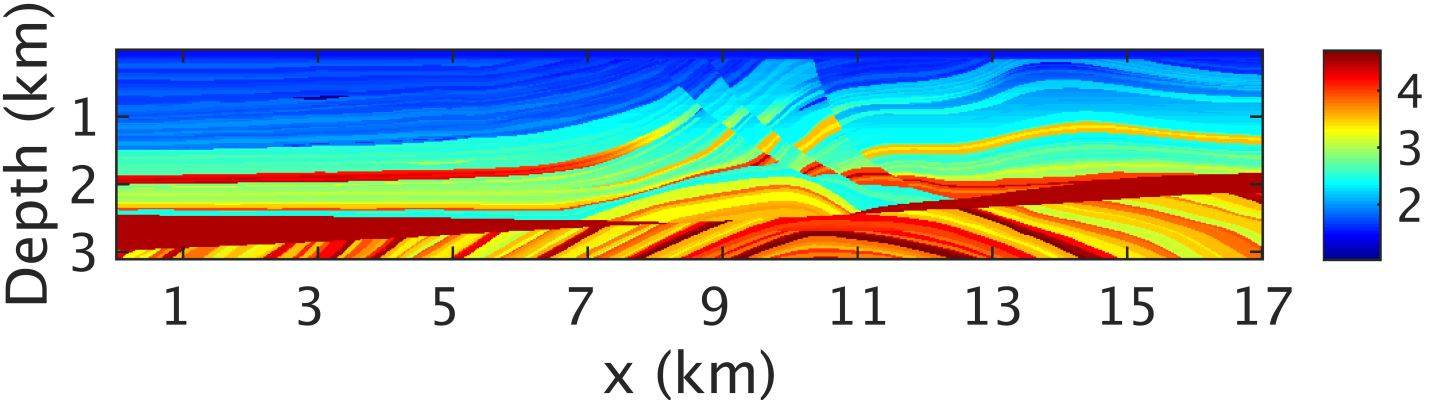
\includegraphics[scale=0.45,trim=0 25 0 0, clip]{101.png} \label{fig:101a}}
\subfloat[]{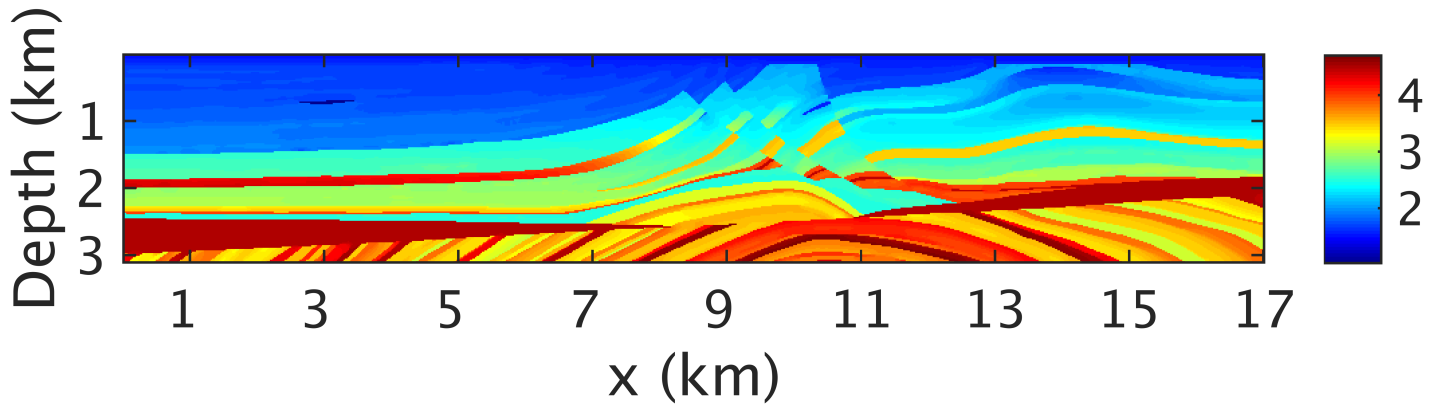
\includegraphics[scale=0.45, trim=25 25 0 0, clip]{102.png} \label{fig:101b}}\\
\subfloat[]{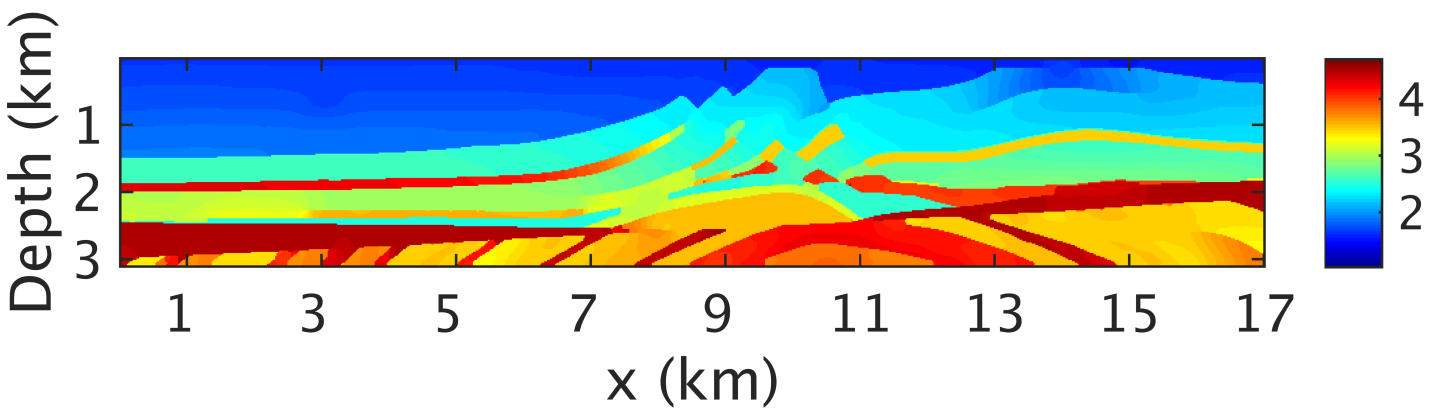
\includegraphics[scale=0.45]{103.png} \label{fig:101c}}
\subfloat[]{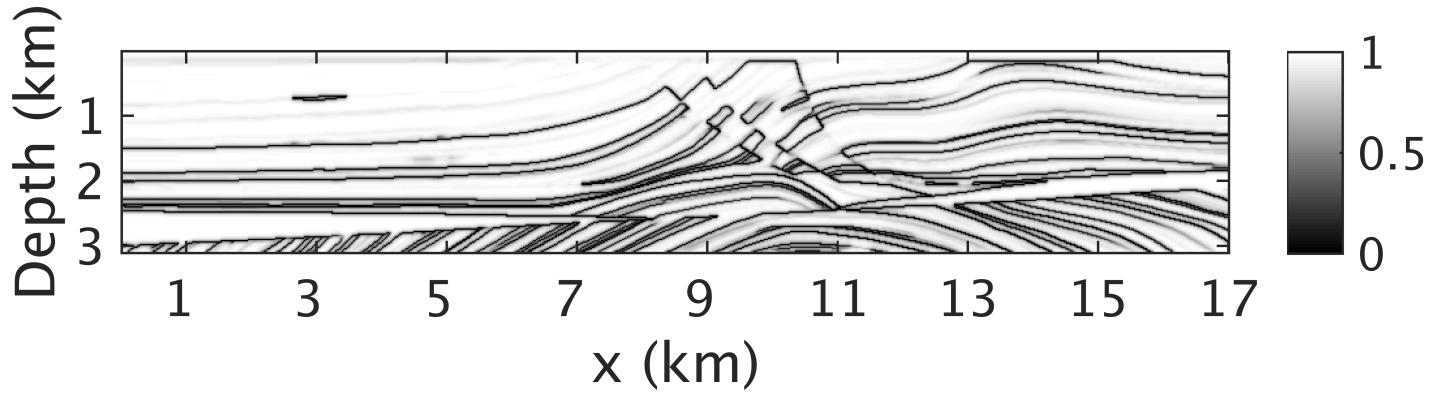
\includegraphics[scale=0.45, trim=25 0 0 0, clip]{104.png} \label{fig:101d}}
    \caption{Reconstructions of Marmousi model using the Mumford-Shah shape representation. (a) Marmousi model~\cite[]{Marmousi2} spanning over $17\times3.1$km domain discretized with $0.02\times0.02$km cells (resulting in an $851\times155$ dimensional discretized domain), (b) Mumford-Shah reconstruction with $\alpha=10$ and $\beta=0.01$, (c) reconstruction with $\alpha=100$ and $\beta=0.01$, and (d) the $\phi_{\epsilon}$ field from the reconstruction with $\alpha=10$.}
\label{fig:101}
\end{figure}
}

\sendatend{
\begin{figure}
\centering
 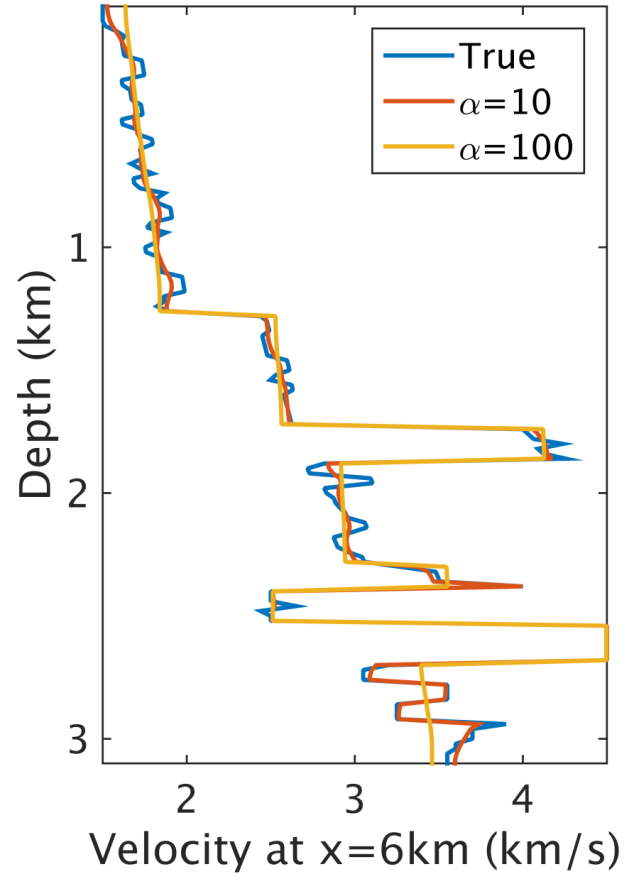
\includegraphics[scale=0.6]{105.png}
\caption{Comparisons of Mumfard-Shah reconstructions with $\alpha=10$ and $\alpha=100$ to the true model at $x=6$km vertical slice.}
 \label{fig:102}
\end{figure}
}

\section{Examples}
%\subsection{Mumford-Shah}
%\textbf{Example} 

\subsection{Subsurface Representation}

Our first example illustrates the ability of the Mumford-Shah inversion technique to segment the Marmousi model into a large number of shapes and interfaces.  Because this example does not incorporate geophysical data, there is actually no inversion taking place.  Instead, we perform image processing (specifically image segmentation) on the Marmousi wave speed model subject to various choices of parameters in the Mumford-Shah functional  (\ref{eq:MS}).

Figure~\ref{fig:101a} illustrates the Marmousi model~\cite[]{Marmousi2} spanning over $17\times3.1$km domain discretized with $0.02\times0.02$km size cells. This discretization results in an $851\times155$ dimensional discretized domain. In order to segment this model into shapes and interfaces, we use the Ambrosio-Tortorelli approximation described in equation~\ref{eq:epsilon}, set $F(\kappa)=\left\vert \nabla \kappa \right\vert^2$, and employ an inexact Gauss-Newton optimization scheme.  In addition, we set $\bar{u}$ to be the Marmousi wave speed model (see~\ref{fig:101a}) and set $u(\kappa)=\kappa$. 

Figures~\ref{fig:101b} and~\ref{fig:101c} illustrate the recovered velocity $\kappa$ when $\alpha$ is set to 10 and 100, respectively while $\beta$ is kept at 0.01. By insepction, we see that the choice of $\alpha = 100$ associated with Figure \ref{fig:101c} results in a smoother velocity model with fewer boundaries. Figure~\ref{fig:101d} illustrates the diffuse interface set $\phi_\epsilon \approx 0$ for the choice $\alpha = 10$; the boundaries between regions correspond to the black lines.

Figure~\ref{fig:102} displays one-dimensional plots of the true and recovered velocities from Figures~\ref{fig:101a}-~\ref{fig:101c} at $x = 6$ km. Figure~\ref{fig:102} confirms that the recovered velocity is smoother when $\alpha = 100$ than when $\alpha = 10$. This observation is true in general: setting the constant $\alpha$ at a high value results in smoother inverted parameter values and fewer boundaries. Therefore, if a detailed image of a subsurface region is desired, the constant $\alpha$ must be kept small. 

\sendatend{
\begin{figure}
\centering 
\subfloat[]{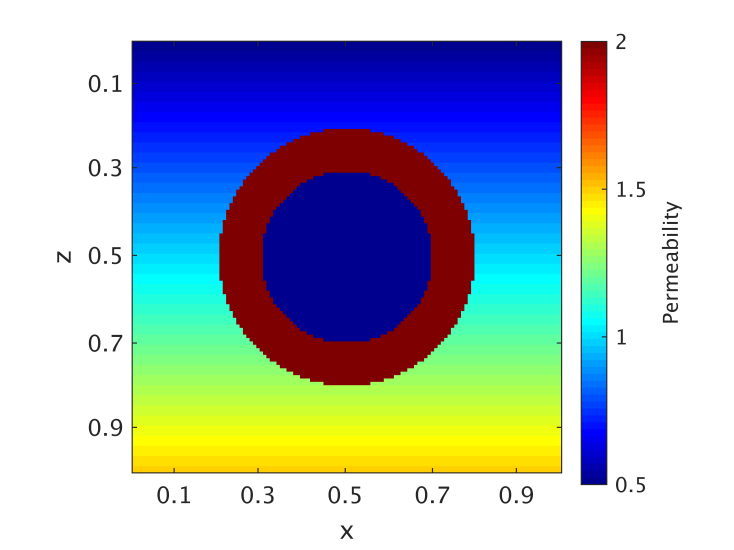
\includegraphics[scale=0.6,trim=0 0 0 0, clip]{201.png} \label{fig:201a}}
\subfloat[]{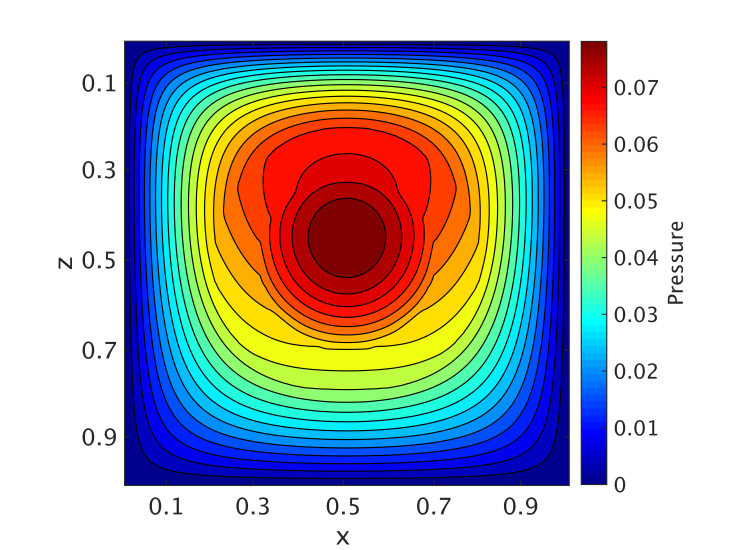
\includegraphics[scale=0.6, trim=0 0 0 0, clip]{202.png} \label{fig:201b}}
\caption{(a) True isotropic permeability field and (b) the pressure profile obtained from this permeability field.}
\label{fig:201}
\end{figure}
}

\subsection{One-phase Flow}

Flow in porous media is important in a wide variety of applications such as reservoir engineering, carbon sequestration, and nuclear waste disposal.  However, due to the wide range of length scales present in the subsurface, it is often prohibitively expensive to simulate transport at the pore scale on which continuum fluid mechanics is valid.  Instead, practical models typically solve for upscaled quantities that are defined at the pore network length-scale.  Central to the upscaling process is the permeability tensor, which provides a simple linear relationship between fluid flux and pressure drop.

Our knowledge of the permeability tensor is inherently imperfect due to our limited ability to access the subsurface.  As a result, for many applications it is necessary to calibrate the permeability tensor with respect to various measured geophysical data (e.g. pressure measurements or production rates).  The development of improved methods for integrating such data sets into reservoir models represents an active area of research in the petroleum engineering community.  

The next two examples consider the inversion of the permeability tensor of a subsurface region from pressure measurements taken throughout the region (i.e., $M=\Omega$). For these examples, all physical quantities, such as pressure and permeability, are assumed to be non-dimensionalized.  For each Mumford-Shah inversion, we use the Ambrosio-Tortorelli approximation described in equation~\ref{eq:epsilon}, set $F(\kappa)=\left\vert \nabla \kappa \right\vert^2$.  Each of the cell-based inversions consists of the minimization of equation~\ref{eq:objective}.  For both inversion techniques, we use a regular Cartesian mesh and optimize using inexact Gauss-Newton.  In these two examples, ten iterations of inexact Gauss-Newton are used.  

\begin{comment}
Next, three numerical examples are studied to compare the Mumford-Shah-based inversion technique to the conventional cell-based inversion technique discussed above. Each of the Mumford-Shah-based inversions consists of the minimization of equation~\ref{eq:shape} using the Ambrosio-Tortorelli approximation as described in equation~\ref{eq:epsilon} and the regularization function $F$ of equation~\ref{eq:Tikhonov}.  Each of the cell-based inversions consists of the minimization of equation~\ref{eq:objective}.  All minimizations are carried out on a regular Cartesian mesh discretization using inexact Gauss-Newton.  In the first two examples, ten iterations are used; for the third example, fifty iterations are used.  For convenience, all of the examples presented here are two dimensional.  However, Mumford-Shah-based inversion may be carried out in any number of spatial dimensions using the procedure described above.  
\end{comment}

Our first example is based on the permeability field found in figure~\ref{fig:201a} and the associated pressure profile found in Figure~\ref{fig:201b}.  Pressure is defined according to equation~\ref{eq:onephase} and a Dirichlet boundary condition
\begin{equation} \label{eq:onephase}
-\nabla \cdot \left( \kappa (x)\nabla p(x) \right)=s(x).
\end{equation}
The source term $s(x)$ in equation~\ref{eq:onephase} models fluid injection, while the Dirichlet boundary condition on pressure assumes that pressure values at the boundary of the reservoir are known.  For simplicity, $p\vert_{\partial\Omega} \equiv 0$ and $s(x) \equiv 1$ are chosen here. 

For inversion purposes, we assume that measured pressure values throughout the domain are available.  In addition, we use an initial guess of $\kappa(x)=4$.  The Mumford-Shah-inversion additionally uses the initial guess $\phi_\epsilon=1$ (i.e., $\Gamma=\emptyset$).

\sendatend{
\begin{figure}
\centering 
\subfloat[]{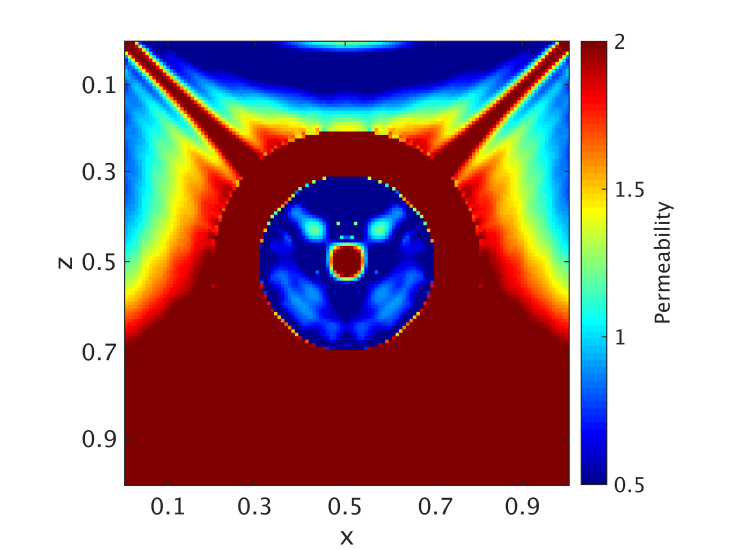
\includegraphics[scale=0.6,trim=0 0 0 0, clip]{203.png} \label{fig:203a}}
\subfloat[]{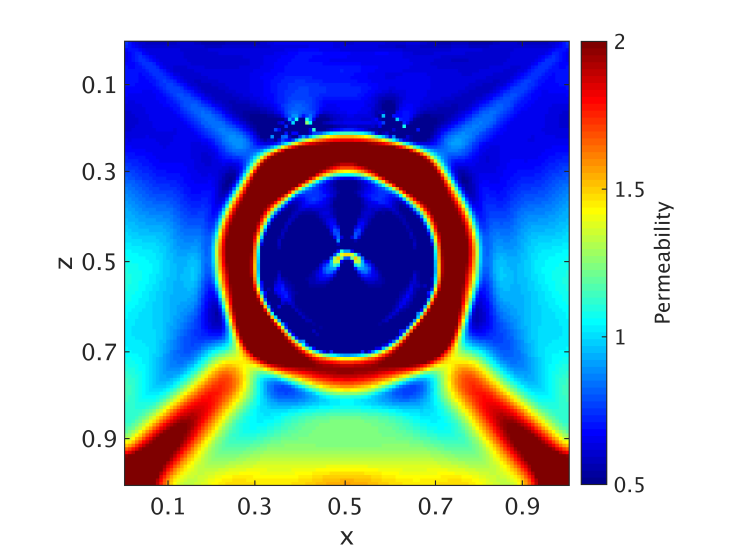
\includegraphics[scale=0.6, trim=0 0 0 0, clip]{204.png} \label{fig:203b}}
\caption{Permeability fields resulting from two conventional cell-based inversion techniques, (a) one without and (b) the other with a Tikhonov regularization term.}
\label{fig:203}
\end{figure}
}

Figure~\ref{fig:203} illustrates permeability fields resulting from two conventional cell-based inversion techniques, one without regularization and the other with Tikhonov regularization.  While the cell-based inversion technique without the regularization term recovers some of the large-scale features of the original model, it also contains high-frequency artifacts and does not properly capture the smooth background permeability field. The addition of Tikhonov regularization stabilizes the cell-based inversion technique.  However, the resulting permeability field smears out the background and the boundaries of the annular region. 

\sendatend{
\begin{figure}
\centering 
\subfloat[]{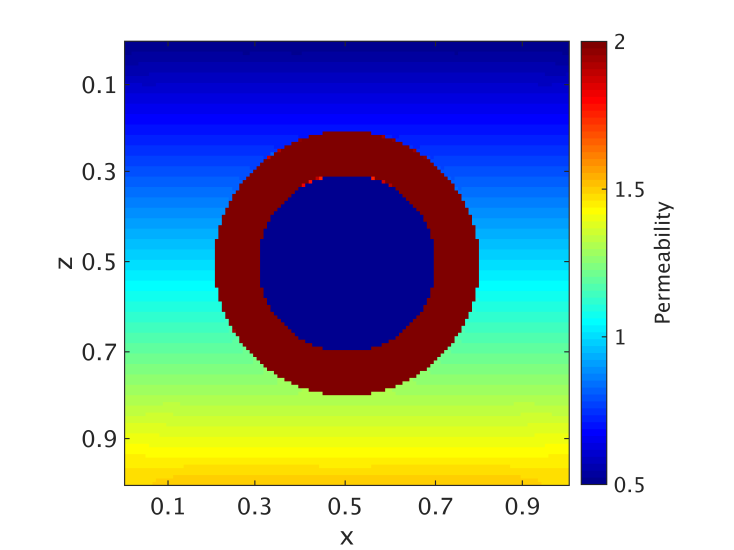
\includegraphics[scale=0.6,trim=0 0 0 0, clip]{205.png} \label{fig:205a}}
\subfloat[]{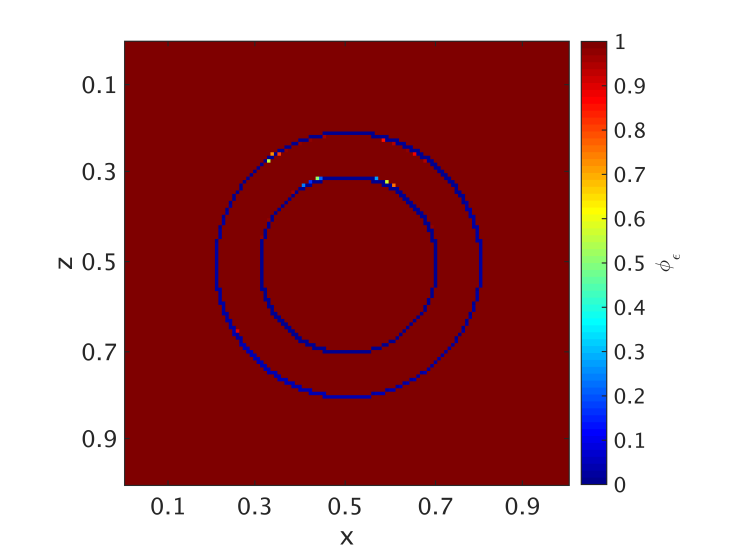
\includegraphics[scale=0.6, trim=0 0 0 0, clip]{206.png} \label{fig:205b}}
\caption{(a) The inverted permeability field and (b) the interface set $\phi_\epsilon$ obtained from the Mumford-Shah-based inversion technique.}
\label{fig:205}
\end{figure}
}
Figure~\ref{fig:205} illustrates the permeability field and the order parameter $\phi_\epsilon$ resulting from the Mumford-Shah-based inversion technique.  There are two aspects of this result worth pointing out.  First, the original permeability field is stably recovered. Second, the interfaces separating regions of smoothness are correctly identified by the zero contour of $\phi_\epsilon$.

\sendatend{
\begin{figure}
\centering
 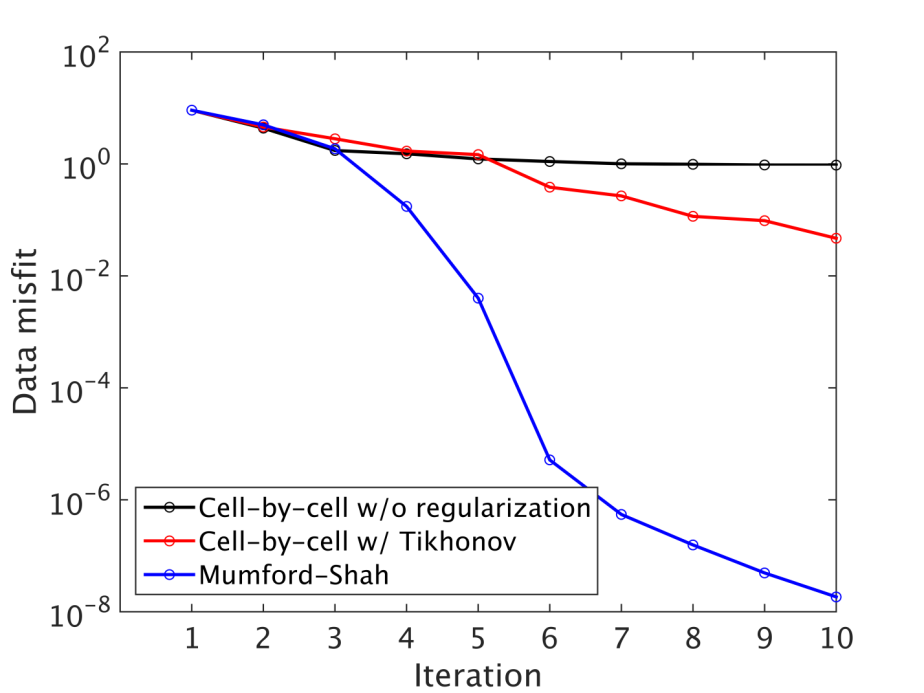
\includegraphics[scale=0.6]{207.png} 
\caption{Comparing data misfits versus number of iterations for the cell-based and Mumfard-Shah inversion techniques.}
\label{fig:207}
\end{figure}
}

Figure~\ref{fig:207} compares the data misfit (using a logarithmic scale) versus the number of iterations for the cell-based and the Mumford-Shah-based inversions.  The Mumford-Shah inversion quickly converges to the correct model whereas the data misfit for the cell-based inversions decreases at a significantly slower rate.

\sendatend{
\begin{figure}
\centering 
\subfloat[]{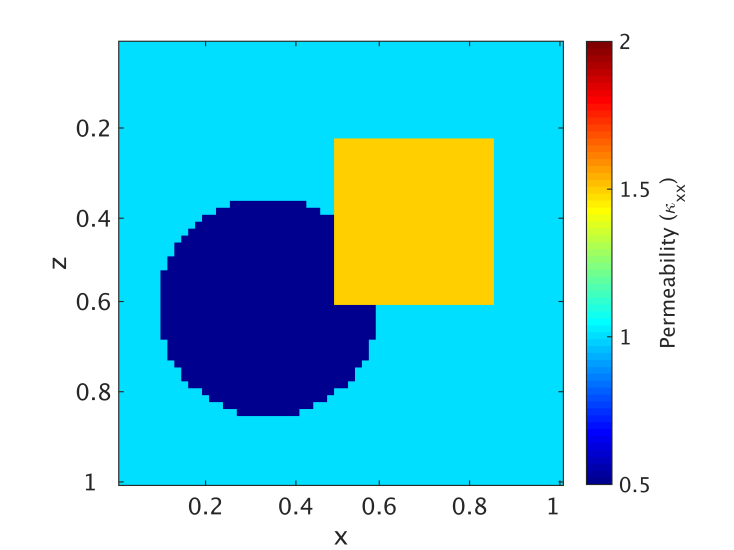
\includegraphics[scale=0.6, trim=0 0 0 0, clip]{208.png} \label{fig:208a}}
\subfloat[]{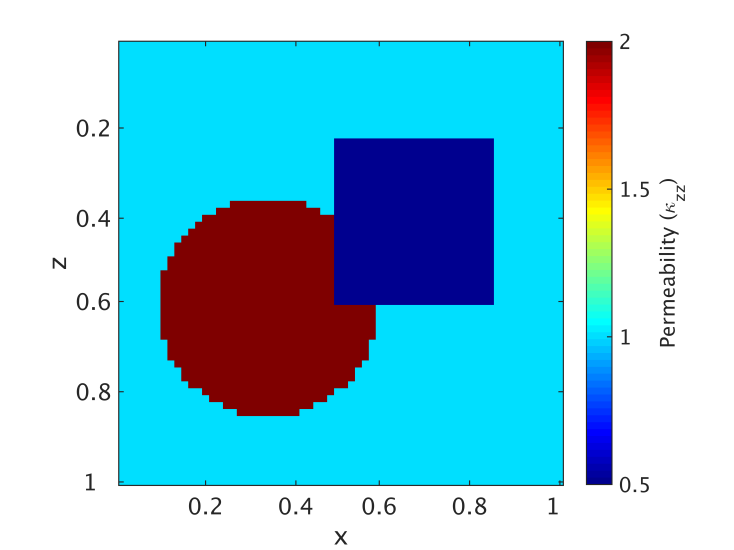
\includegraphics[scale=0.6, trim=0 0 0 0, clip]{209.png} \label{fig:208b}}
\subfloat[]{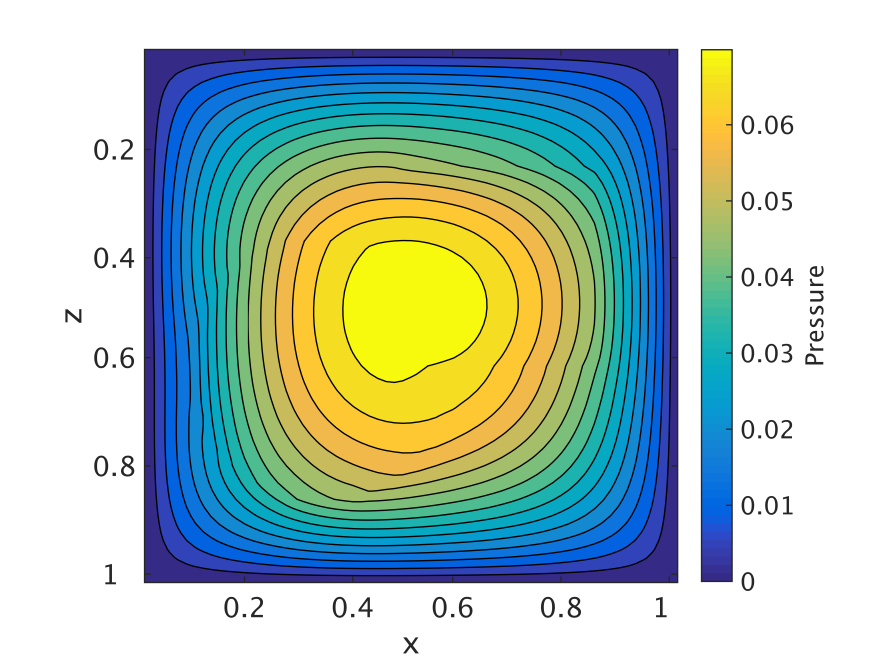
\includegraphics[scale=0.5, trim=0 0 0 0, clip]{210.png} \label{fig:208c}}
\caption{The true anisotropic permeability fields (a) $\kappa_{xx}$ and (b) $\kappa_{zz}$, and the pressure field obtained using equation~\ref{eq:onephase} and permeability fields from (a) and (b).}
\label{fig:208}
\end{figure}
}

\subsection{Multi-parameter One-phase Flow}
For our next example, we seek to identify an anisotropic permeability tensor from the associated fluid pressure measurements.  In practice, anisotropy of the permeability tensor is common and is a natural consequence of the layered nature of the subsurface.  As a result, horizontal permeability values often differ from vertical ones.

Our next example is based on the anisotropic permeability model displayed in Figures~\ref{fig:208a} and~\ref{fig:208b}.  Due to anisotropy, $\kappa_{xx} \neq \kappa_{zz}$; however, $\kappa_{xx}$ and $\kappa_{zz}$ do share a common set of interfaces.  As in the previous example, the pressure profile (see Figure ~\ref{fig:208c}) is  computed by solving equation~\ref{eq:onephase} using the zero Dirichlet boundary condition and $s(x) \equiv 1$.  

For inversion purposes, we assume that measured pressure values throughout the domain are available.  In addition, we use an initial guess of $\kappa_{xx}=\kappa_{zz}=1$.  The Mumford-Shah-inversion additionally uses the initial guess $\phi_\epsilon=1$ (i.e., $\Gamma=\emptyset$).

\sendatend{
\begin{figure}
\centering 
\subfloat[]{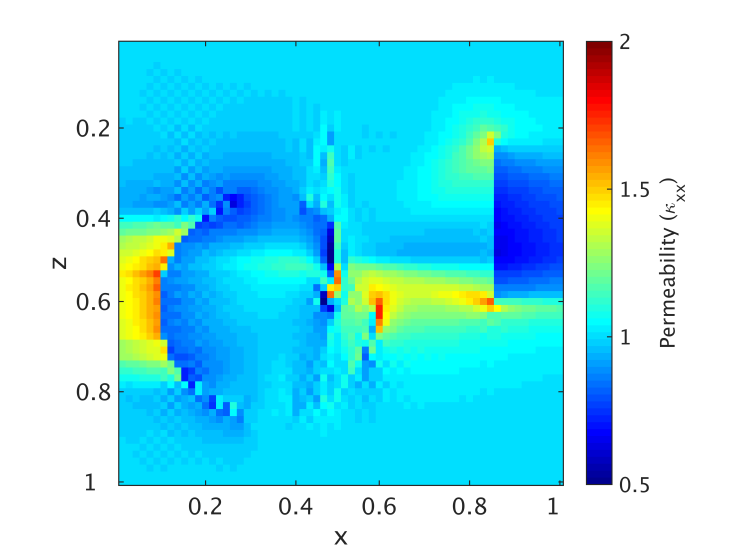
\includegraphics[scale=0.6, trim=0 0 0 0, clip]{211.png} \label{fig:211a}}
\subfloat[]{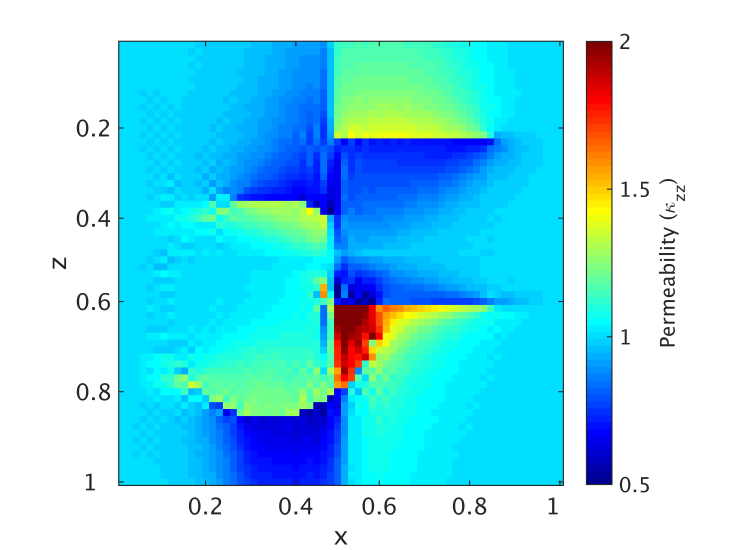
\includegraphics[scale=0.6, trim=0 0 0 0, clip]{212.png} \label{fig:211b}}
\caption{The inverted anistropic permeability fields (a) $\kappa_{xx}$ and (b) $\kappa_{zz}$ resulting from the conventional cell-based inversion.}
\label{fig:211}
\end{figure}
}

Figure~\ref{fig:211} illustrates the permeability tensor resulting from the cell-based inversion without regularization.  Since the cell-based inversion formulation does not enforce a spatial correlation between the inverted tensor components, the result is non-unique and unstable.  In contrast, the inverted permeability tensor based on Mumford-Shah is well-structured and the interface set is correctly identified (see Figure~\ref{fig:213}).  

\sendatend{
\begin{figure}
\centering 
\subfloat[]{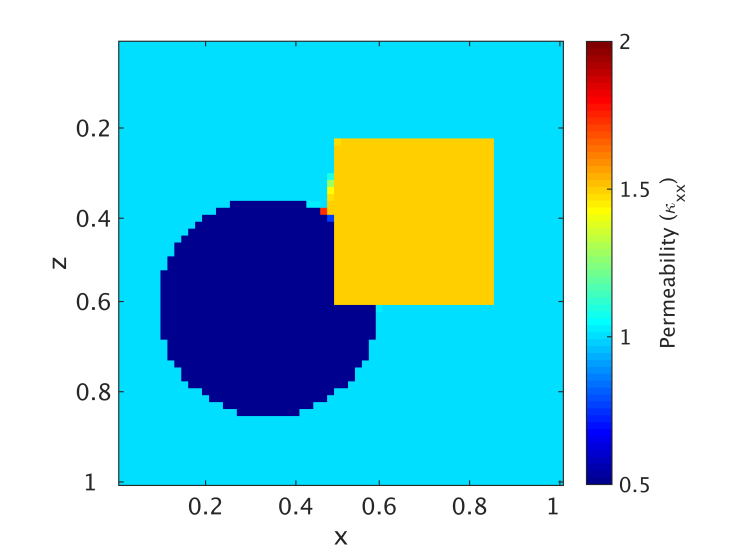
\includegraphics[scale=0.6, trim=0 0 0 0, clip]{213.png} \label{fig:213a}}
\subfloat[]{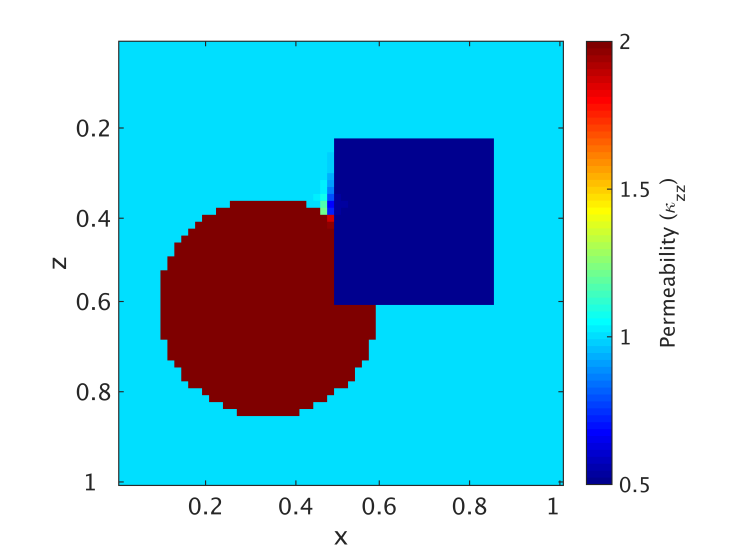
\includegraphics[scale=0.6, trim=0 0 0 0, clip]{214.png} \label{fig:213b}}
\subfloat[]{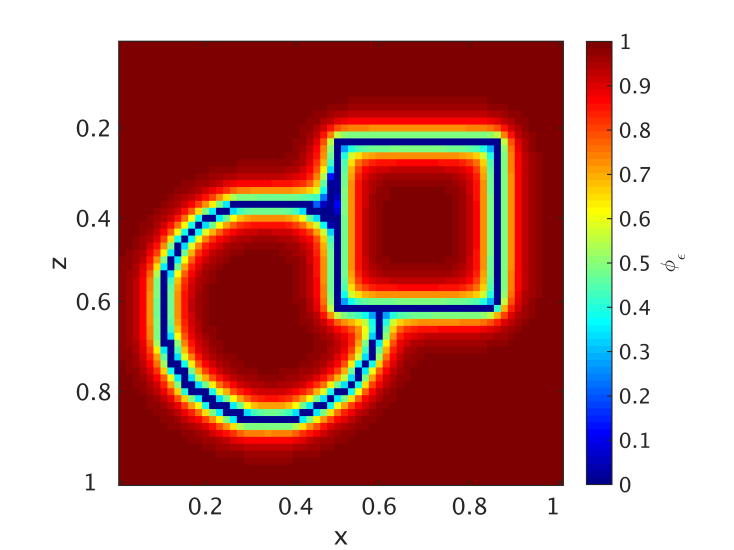
\includegraphics[scale=0.6, trim=0 0 0 0, clip]{215.png} \label{fig:213c}}
\caption{The inverted permeability tensor components (a) $\kappa_{xx}$, (b) $\kappa_{zz}$, and (c) the interface set $\phi_\epsilon$ resulting from the Mumford-Shah-based inversion.}
\label{fig:213}
\end{figure}
}
\sendatend{
\begin{figure}
\centering
 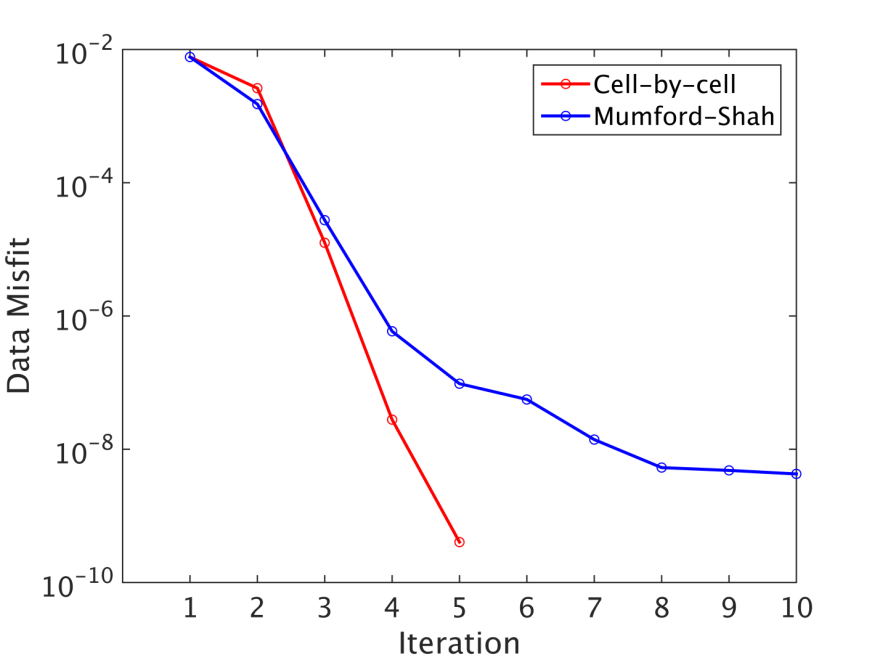
\includegraphics[scale=0.6]{216.png}
\caption{Comparing data misfit versus number of iterations for the cell-based and Mumfard-Shah inversion techniques.}
 \label{fig:216}
\end{figure}
}
Figure~\ref{fig:216} compares the data misfit (on a logarithmic scale) versus the number of iterations for the above results.  Interestingly, both inversions match the data.  This highlights the utility of Mumford-Shah as a regularization scheme that enforces spatial correlations between parameters.  

\sendatend{
\begin{figure}
\centering 
\subfloat[]{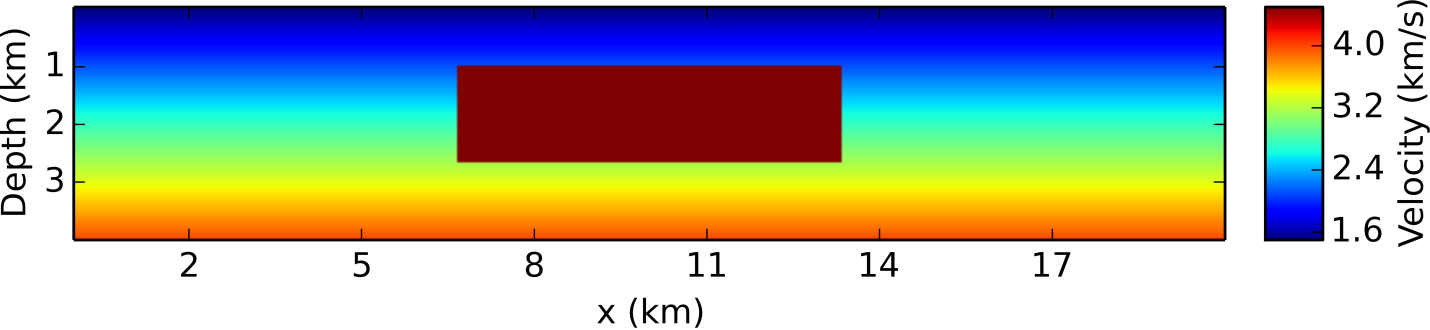
\includegraphics[scale=0.6, trim=0 0 0 0, clip]{301.png} \label{fig:301a}} \\
\subfloat[]{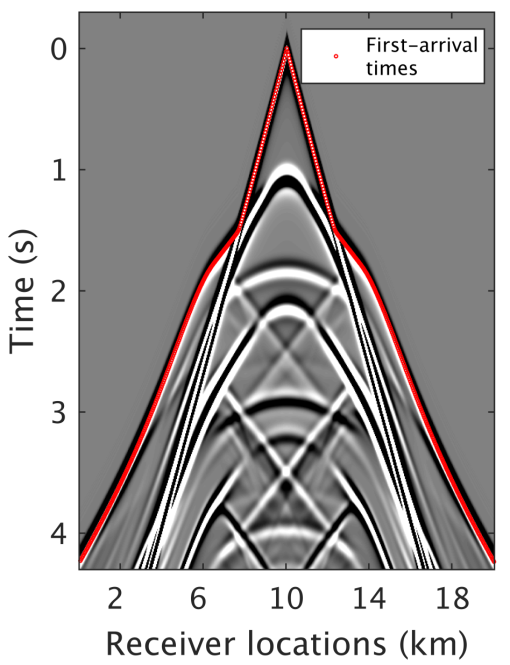
\includegraphics[scale=0.6, trim=0 0 0 0, clip]{302.png} \label{fig:301b}}
\subfloat[]{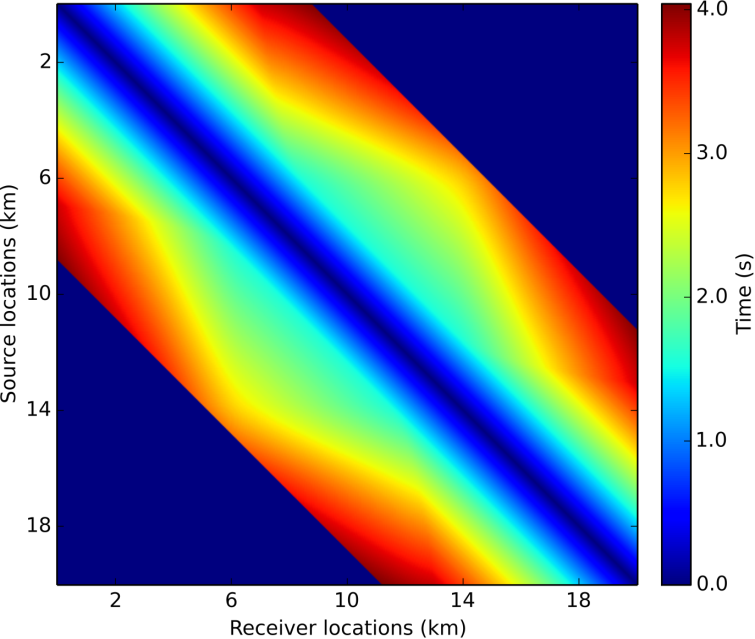
\includegraphics[scale=0.6, trim=0 0 0 0, clip]{303.png} \label{fig:301c}}
\caption{(a) A block velocity model with a linearly sloping background velocity model and (b) seismogram obtained for a source located in the middle of the model and set of 501 receivers spreaded over the surface, and (c) the first-arrival data for 501 sources and 501 receivers spreaded over the surface. The red dots on (b) corresponds to the first-arrival times on the seismogram.}
\label{fig:301}
\end{figure}
}

\subsection{First-arrival Travel Time Tomography}
For our next example, we recover the location of an anomalous homogeneous body using first-arrival travel time data.  The subsurface model in this case is illustrated in Figure~\ref{fig:301a}.  The anomalous body is a rectangular region with constant wave speed of 4.5 km/s.  The background wave speed, linearly-varying, is equal to 1.5 km/s at the top surface (depth = 0 km) and 4.0 km/s at a depth = 4 km.  Five hundred and one seismic sources and five hundred and one seismic receivers are placed equidistantly on the top surface of the region from x = 0 km to 20 km. In consideration of realistic seismic surveys such as towed-streamer seismic acquisition, each receiver is limited to listening to sources within 10 km.  In other words, the maximum source-receiver offset is 10 km.   An example of a seismogram, due to a source located at x = 10 km, is shown in Figure~\ref{fig:301b}; the red line corresponds to the first-arrival times.

\sendatend{
\begin{figure}
\centering 
\subfloat[]{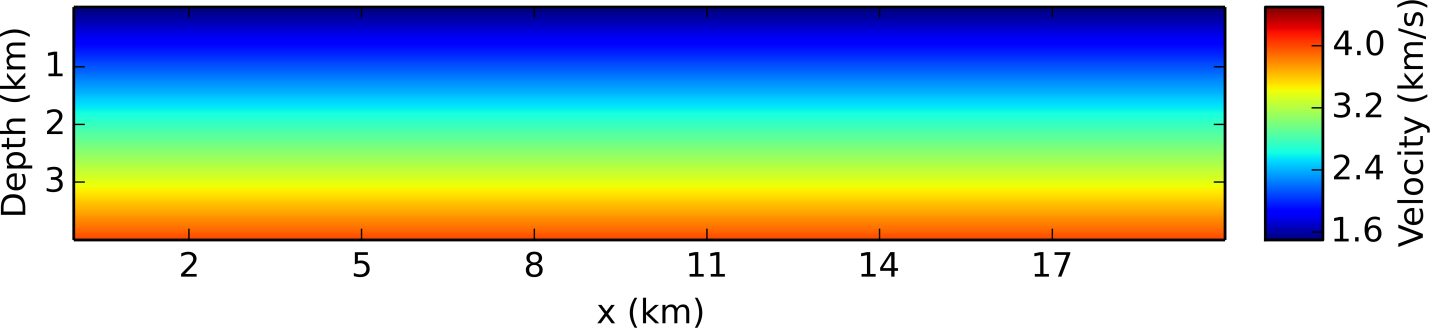
\includegraphics[scale=0.45,trim=0 12 0 0, clip]{304.png} \label{fig:304a}}
\subfloat[]{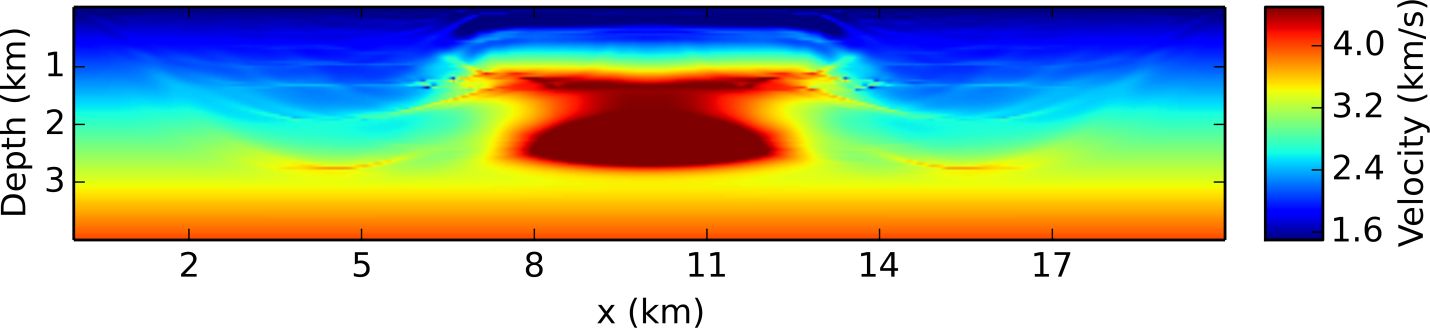
\includegraphics[scale=0.45, trim=12 12 0 0, clip]{305.png} \label{fig:304b}}\\
\subfloat[]{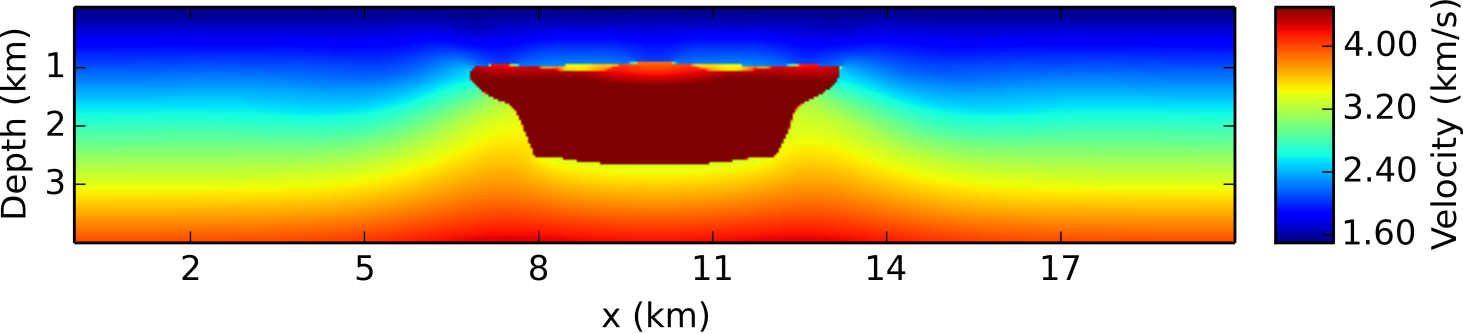
\includegraphics[scale=0.45]{306.png} \label{fig:304c}}
\subfloat[]{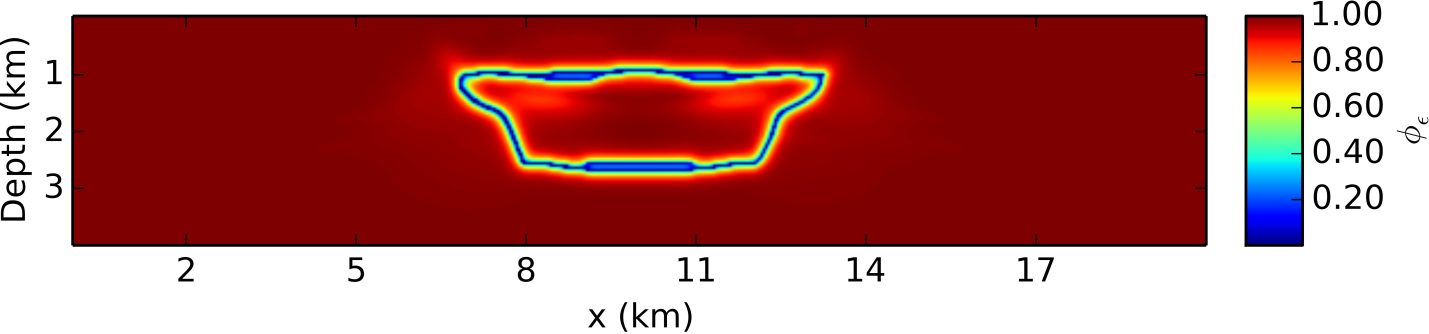
\includegraphics[scale=0.45, trim=12 0 0 0, clip]{307.png} \label{fig:304d}}
\caption{(a) The background velocity model as the initial guess, (b) the velocity model inverted using the conventional cell-based inversion, (c) the velocity model inverted using Mumford-Shah inversion, and (d) the boundary set obtained from Mumford-Shah inversion. }
\label{fig:304}
\end{figure}
}

The available data in this example are the first-arrival times associated with the 501 sources and 501 receivers, as illustrated in Figure~\ref{fig:301c}.  First-arrival travel times T for both data generation and inversion are computed by solving the Eikonal equation
\begin{equation} \label{eq:eikonal}
\left\vert \nabla T \right\vert = \frac{1}{\kappa} 
\end{equation}
with the boundary condition $T\vert_{\Gamma_S}=0$ at the source locations $\Gamma_S$ and the spatially varying wave speed $\kappa$ as given. Equation~\ref{eq:eikonal} is solved by the fast sweeping method~\cite[]{Zhao04}. 

The initial guess for the conventional cell-based inversion technique is the background wave speed profile illustrated in Figure~\ref{fig:304a}.  The initial guess for the Mumford-Shah inversion is the background wave speed profile and $\phi_\epsilon=1$ (i.e., $\Gamma=\emptyset$).  Fifty iterations of inexact Gauss-Newton are used for the cell-based and Mumford-Shah inversions.  

The wave speed from the cell-based inversion is illustrated in Figure~\ref{fig:304b}.  Note that no regularization is included.  The wave speed and inverted interface set $\phi_\epsilon$ from the Mumford-Shah inversion are illustrated in Figure~\ref{fig:304c} and Figure~\ref{fig:304d}, respectively.  A comparison of Figures~\ref{fig:304b} and ~\ref{fig:304c} indicates that the wave speed recovered by Mumford-Shah represents an improvement over the cell-based inversion method.

\sendatend{
\begin{figure}
\centering 
\subfloat[]{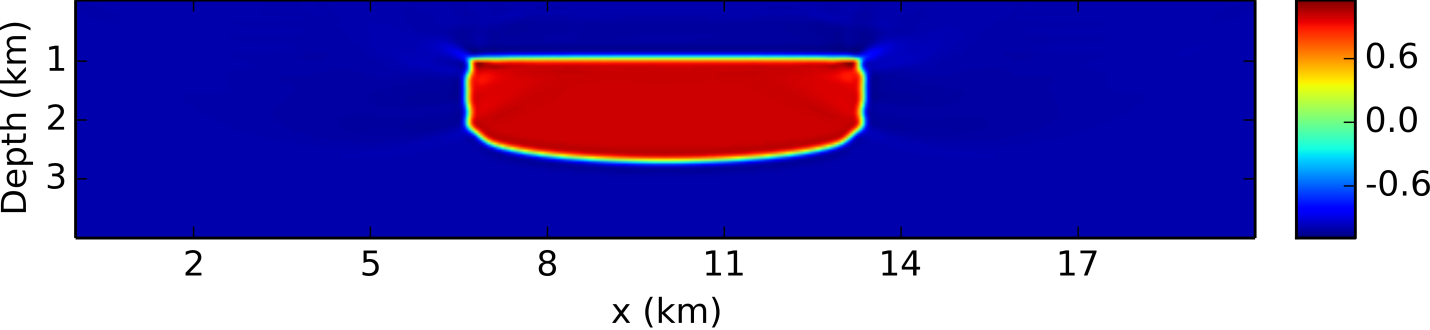
\includegraphics[scale=0.45, trim=0 0 0 0, clip]{401.png} \label{fig:401a}}
\subfloat[]{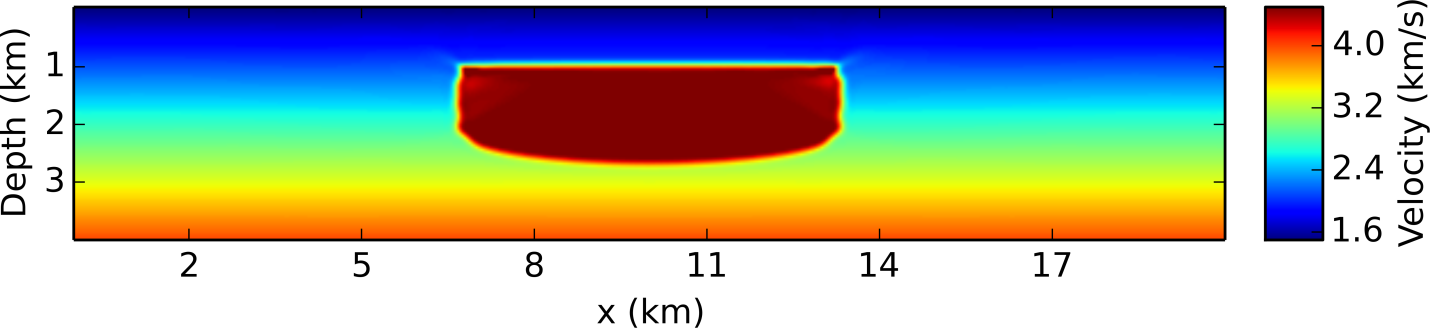
\includegraphics[scale=0.45, trim=0 0 0 0, clip]{402.png} \label{fig:401b}}
\caption{(a) The phase-field function $\phi_\epsilon$ resulting from phase-field inversion and (b) is the corresponding velocity model using equation~\ref{eq:pf_kappa}}
\label{fig:401}
\end{figure}
}

However the anomalous target is not fully recovered by Mumford-Shah inversion as observed from Figure~\ref{fig:304c}. To improve the Mumford-Shah inversion results, we make use of the phase-field method. We will attempt to determine the location of the same anomalous body using phase-field method with the same first-arrival travel time data illustrated in Figure~\ref{fig:301}.

This phase-field inversion optimizes equation~\ref{eq:pf_epsilon} using the representation of $\kappa$ given by equation~\ref{eq:pf_kappa}. The inversion is performed on a regular Cartesian mesh using fifty iterations of inexact Gauss-Newton similar to the previous Mumford-Shah inversion. The initial guess is the same background wave speed profile illustrated in Figure~\ref{fig:304a}; for phase-field, this amounts to an initial guess of $\phi=-1$.  For phase-field, we assume the parameters values $\kappa_i$ in equation~\ref{eq:pf_kappa} are fixed and only infer for the phase-field function $\phi$ which partitions the subsurface into two shapes $\{\Omega_1,\Omega_2 \}$. The domain $\Omega_1$ represents the anomalous body and the domain $\Omega_2$ represents the surrounding background. The parameter value $\kappa_1$ represents the wave speed within the anomalous body and is fixed at 4.5 km/s. The parameter value $\kappa_2$ is fixed to be the background wave speed profile, as shown in Figure~\ref{fig:304a}.

Figure~\ref{fig:401b} illustrates the wave speed obtained from phase-field.  This is obtained by plugging in the optimized phase-field function $\phi_\epsilon$, illustrated in Figure~\ref{fig:401a}, into equation~\ref{eq:pf_kappa}.  Figure~\ref{fig:401a} demonstrates that the phase-field function $\phi_\epsilon$ demarcates two shapes with a narrow transition region where $\phi_\epsilon$ transitions from a value of 1 to a value of -1. The phase-field inversion (Figure~\ref{fig:401b}) results in an improved construction of the anomalous target as compared to both the cell-based and Mumford-Shah inversions (Figures~\ref{fig:304b} and~\ref{fig:304c} respectively).

\sendatend{
\begin{figure}
\centering 
\subfloat[]{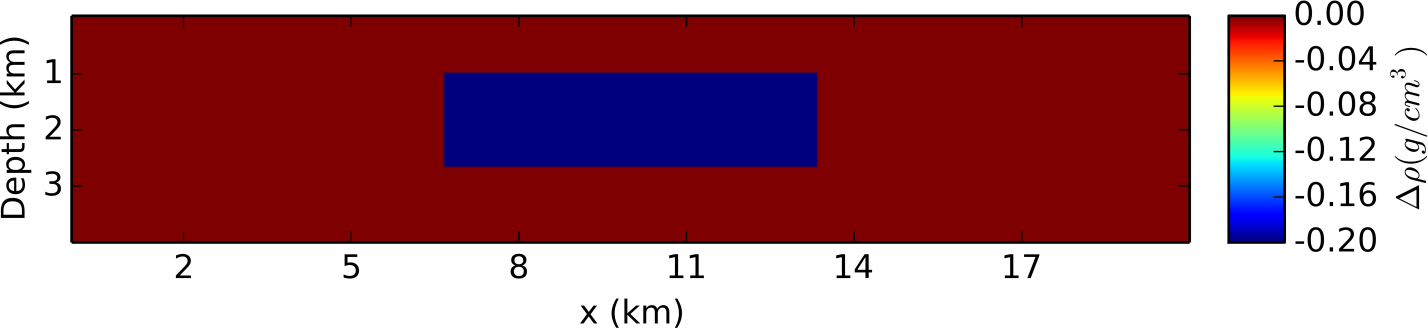
\includegraphics[scale=0.5,trim=0 0 0 -40, clip]{501.png} \label{fig:501a}}
\subfloat[]{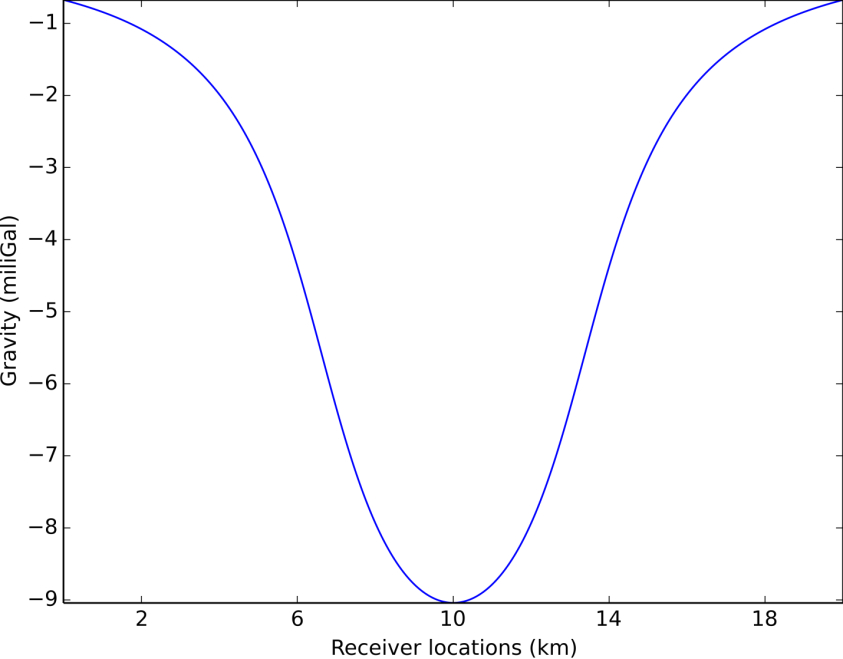
\includegraphics[scale=0.5, trim=0 0 0 0, clip]{502.png} \label{fig:501b}}
\caption{(a) Differential density model ($\Delta\rho$) and (b) surface measurement of gravity based on the density difference model in (a).}
\label{fig:501}
\end{figure}
}

\subsection{Gravity}
This example seeks to determine the location of the same anomaly as the previous example, but this time using only gravity data. 

Gravity data are generated using the subsurface density model illustrated in Figure~\ref{fig:501a}.  The model assumes a uniform background density and an anomalous rectangular region with $-20 g/cm^3$ density difference relative to the background, as shown in Figure~\ref{fig:501a}. In reality, the background density vary in depth, but for the simplicity of this example we assume that it is constant in depth. Both Mumford-Shah and phase-field inversion methods can be employed for any spatial distributions of inversion parameters as already demonstrated. Note that the density and velocity models share the same boundary set, as can be observed from Figures~\ref{fig:301a} and~\ref{fig:501a}.  

\sendatend{
\begin{figure}
\centering 
\subfloat[]{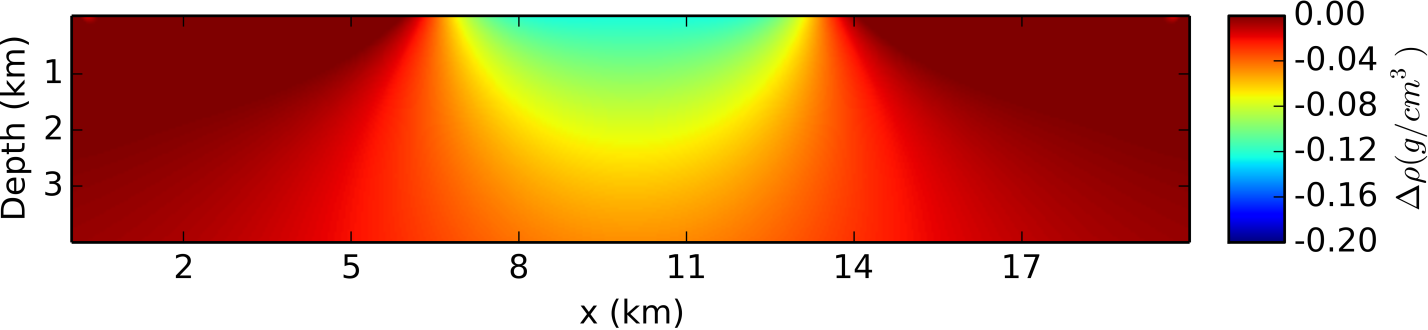
\includegraphics[scale=0.45, trim=0 0 0 0, clip]{503B.png} \label{fig:505a}}
\subfloat[]{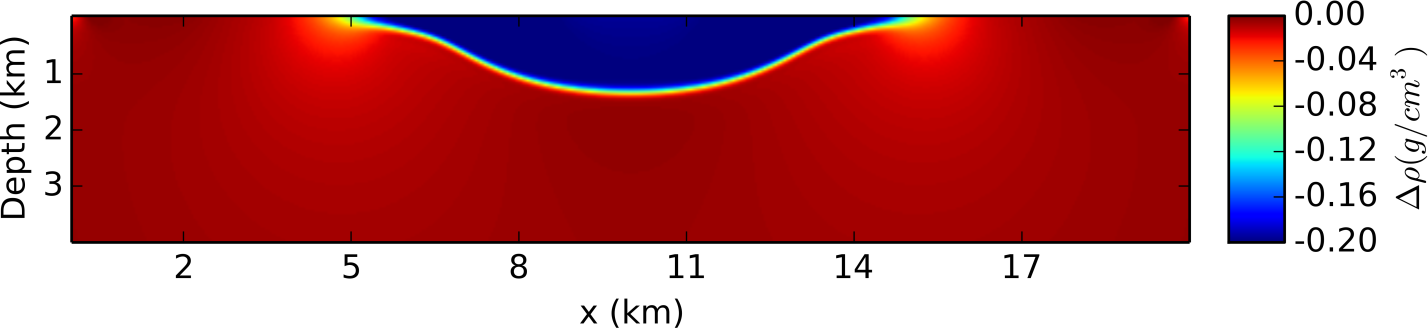
\includegraphics[scale=0.45, trim=0 0 0 0, clip]{506.png} \label{fig:505b}}
\caption{The inversion results from (a) cell-based inversion and (b) phase-field inversion of data provided in Figure~\ref{fig:501b}.}
\label{fig:505}
\end{figure}
}

Gravity anomaly data $g_z$ is generated by solving for the gravitational potential $U$ in equation~\ref{eq:gravity} 
\begin{equation} \label{eq:gravity}
\nabla^2 U = 4 \pi G \Delta \rho
\end{equation}
and using the relationship $g_z=\partial U / \partial z$.  Here, $\nabla^2$ is the Laplacian operator, $G$ is the gravitational constant of $6.67408\times 10^{-11} m^3 kg^{-1} s^{-2}$, and $\Delta \rho$ indicates the spatially varying difference between the subsurface density and the background density.   $\Delta \rho$ is defined by equation~\ref{eq:deltarho} below

\begin{equation} \label{eq:deltarho}
\Delta \rho (x) = \begin{cases} \Delta \rho_a &  \text{if}~x \in \text{anomaly} \\ 0 & \text{if}~x \not\in \text{anomaly} \end{cases}.
\end{equation}

Gravity measurements are made at 501 locations at 300 m above the top surface of the domain.  The gravity measurements for the target model are provided in Figure~\ref{fig:501b}. 

The initial guess for both inversions is the background model (i.e. no presence of the anomaly).  Both optimizations are run for fifty iterations of inexact Gauss-Newton.  Similar to the previous example, the phase-field inversion assumes as known the density anomaly value $\Delta \rho_a$ corresponding to the density increment due to the anomaly associated with domain $\Omega_1$; the remaining unknown is the phase-field function $\phi$ determining the regions $\Omega_1$ and $\Omega_2$. We may compute the density update from the phase-field parameter using equation~\ref{eq:pf_deltarho} below
\begin{equation} \label{eq:pf_deltarho}
\Delta \rho (x)=\frac{1-\phi(x)}{2} \Delta \rho_a.
\end{equation}

Figure~\ref{fig:505a} illustrates the density anomaly resulting from the cell-based inversion; note that no regularization term is included here.  Figure \ref{fig:505b} illustrates the density anomaly resulting from phase-field inversion.  Not surprisingly, neither the conventional cell-based inversion technique nor the phase-field inversion technique accurately locates the anomalous body due to the Laplacian smoothing present in equation~\ref{eq:gravity} and the limited measurements available above the domain.

\sendatend{
\begin{figure}
\centering 
\subfloat[]{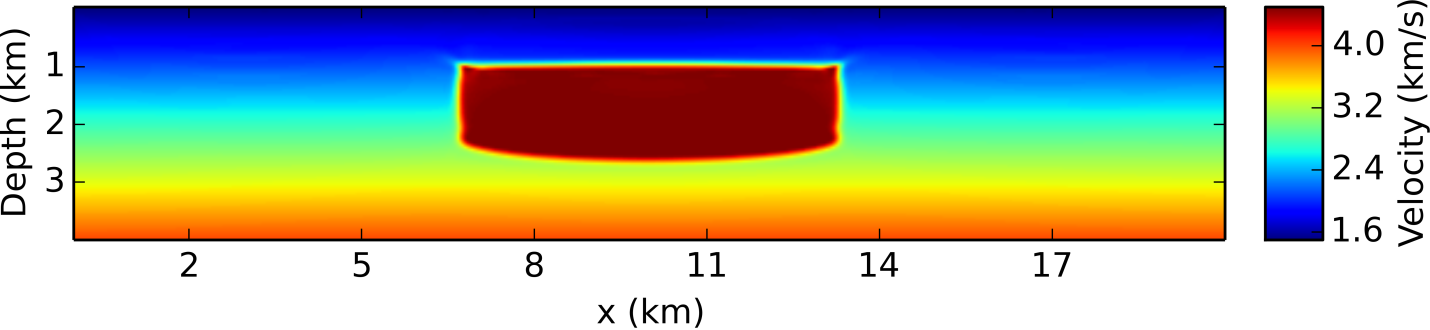
\includegraphics[scale=0.45, trim=0 0 0 0, clip]{601.png} \label{fig:601a}}
\subfloat[]{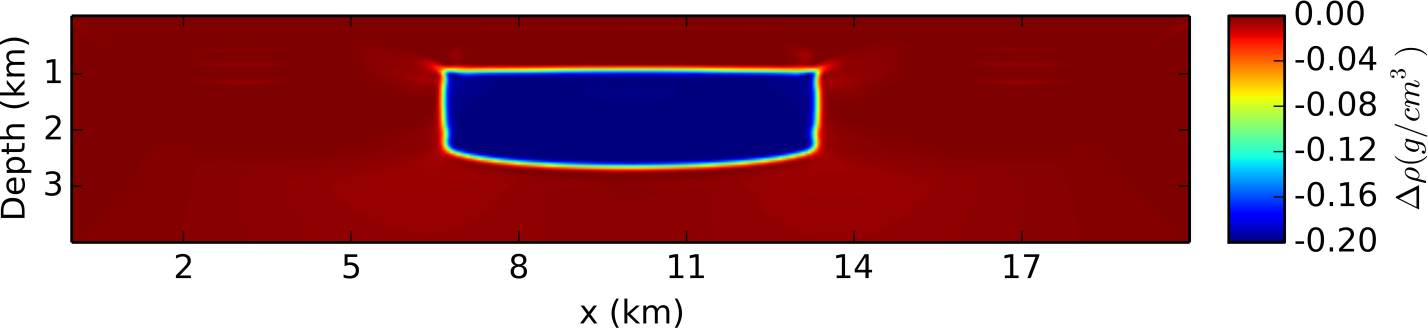
\includegraphics[scale=0.45, trim=0 0 0 0, clip]{602.png} \label{fig:601b}}
\caption{The phase-field inversion results using joint travel-time (Figure~\ref{fig:301c}) and gravity data  (Figure~\ref{fig:501b}) for (a) the wave velocity and (b) differential density.}
\label{fig:601}
\end{figure}
}

\subsection{Joint Travel-time and Gravity}

In this example, we seek to determine the location of the anomalous body using both first-arrival travel time data and gravity data anomaly data. The initial guesses for wave speed (Figure~\ref{fig:301a}) and density (Figure~\ref{fig:501a}) remain unchanged from the earlier examples. 

The density and wave-speed profiles for the cell-based inversion are identical to those obtained in the previous examples since the cell-based approach does not couple density and wave speed.  Figure~\ref{fig:304b} represents the inverted wave speed profile in this case and Figure~\ref{fig:505b} represents the inverted density profile. Figure~\ref{fig:601} displays the inverted wave speed and density profiles for the joint phase-field inversion, along with the phase-field function $\phi_\epsilon$. Joint inversion greatly improves the estimation of density and provides some uplift to wave speed.

\sendatend{
\begin{figure}
\centering 
\subfloat[]{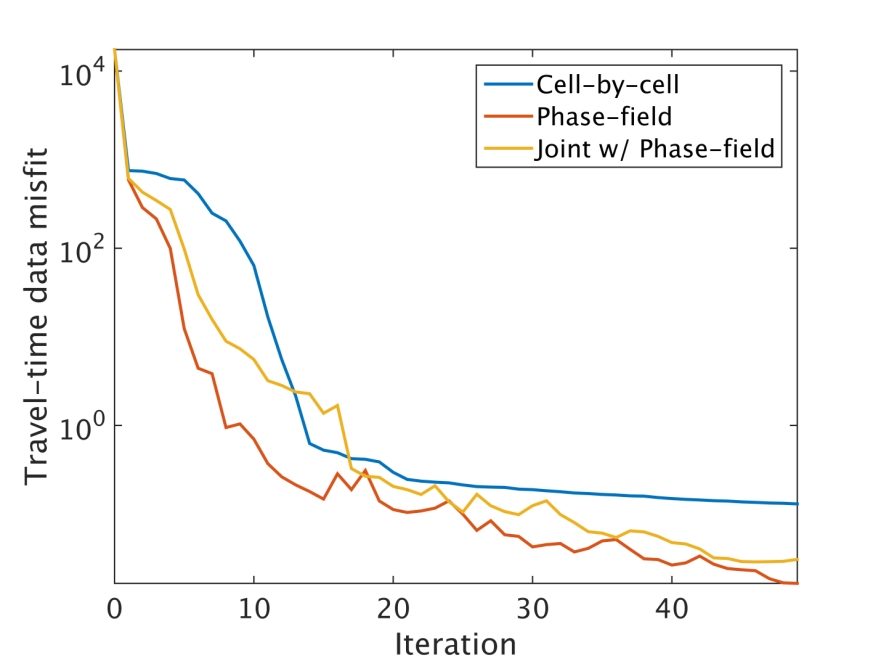
\includegraphics[scale=0.55, trim=0 0 0 0, clip]{604.png} \label{fig:604a}}
\subfloat[]{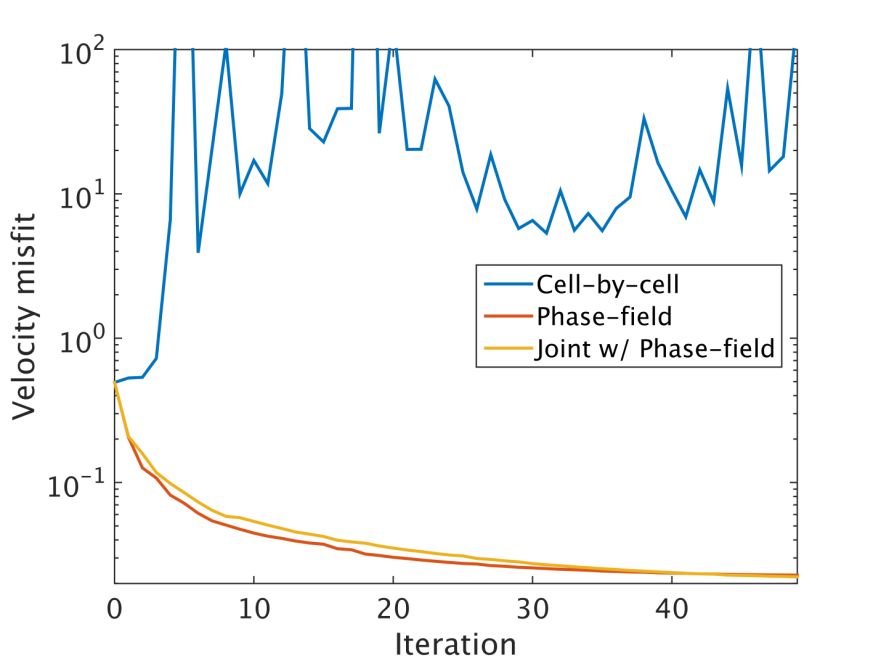
\includegraphics[scale=0.55, trim=0 0 0 0, clip]{605.png} \label{fig:604b}} \\
\subfloat[]{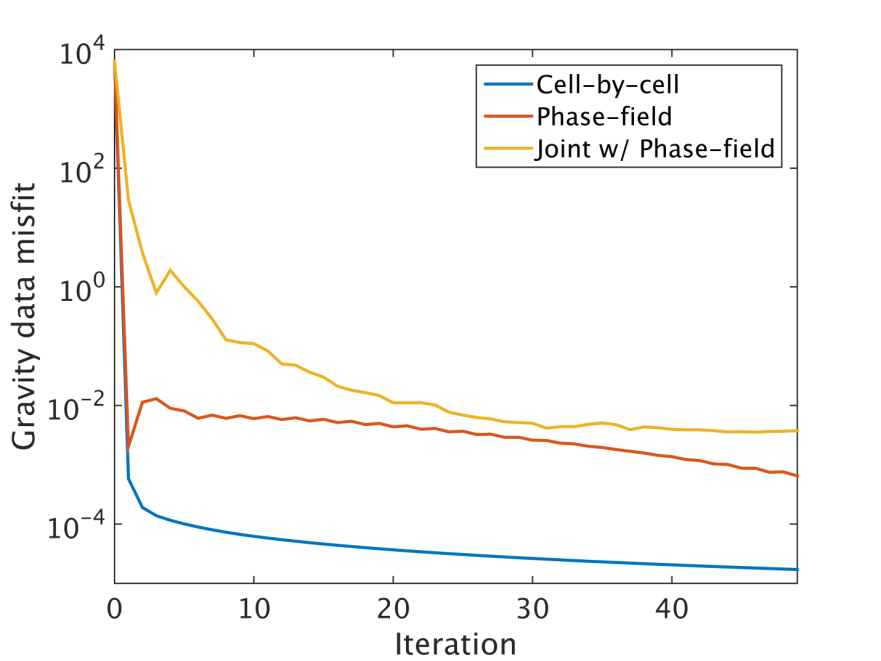
\includegraphics[scale=0.55, trim=0 0 0 0, clip]{606.png} \label{fig:604c}}
\subfloat[]{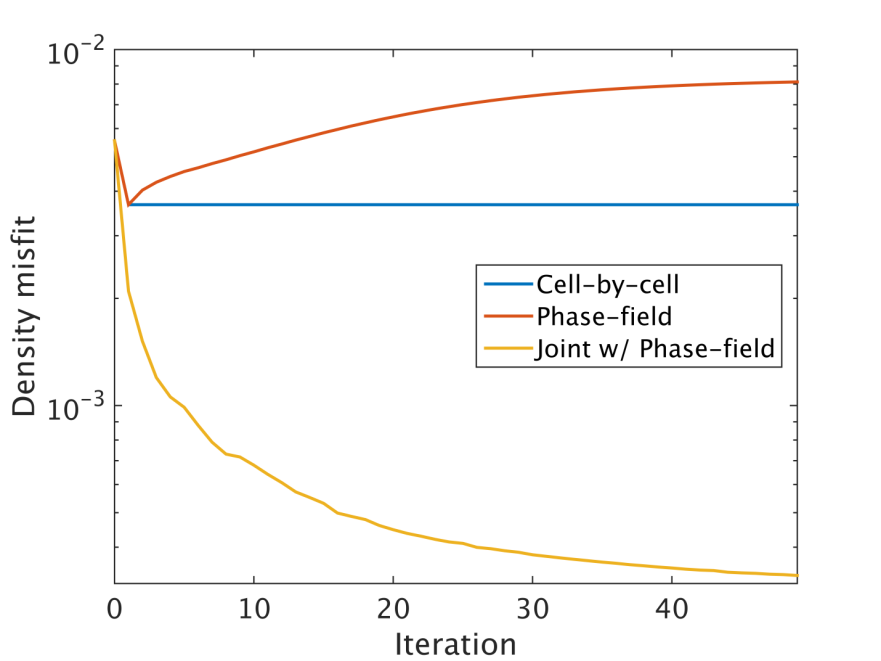
\includegraphics[scale=0.55, trim=0 0 0 0, clip]{607.png} \label{fig:604d}}
\caption{(a) Travel-time data misfit, (b) velocity model misfit, (c) gravity data misfit and (d) density model misfit verus number of iterations for inversions with cell-based and phase-field techniques.}
\label{fig:604}
\end{figure}
}

Figures~\ref{fig:604a} and~\ref{fig:604b} display the first-arrival travel time data misfit and wave speed model misfit versus the number of iterations.  Three aspects of these plots stand out.  First, Figure ~\ref{fig:604a} indicates that the data misfit decreases monotonically for the cell-based inversion but does not for the phase-field inversions.  This is due to the geometric regularization terms present in the phase-field inversion.  As a result, the overall objective in the phase-field inversions decreases monotonically but the data misfit is not guaranteed to do so.   Second, Figure ~\ref{fig:604b} indicates that the model misfit for the phase-field inversions is orders of magnitude smaller than for the cell-based inversion. This can be confirmed visually by comparing Figures~\ref{fig:304b},~\ref{fig:401b}, and~\ref{fig:601a} to the ground truth, Figure~\ref{fig:301a}.  Third, data and model misfit are comparable for phase-field inversion of travel-time data alone and joint phase-field inversion of travel-time and gravity data.   

Figures~\ref{fig:604c} and~\ref{fig:604d} plot the gravity data misfit and density model misfit versus the number of iterations. Two aspects of the plots stand out.  First, Figure~\ref{fig:604d}, demonstrates that the model misfit for the joint phase-field inversion of gravity and travel-time data is significantly smaller than the cell-based approach or the phase-field approach using only gravity data. This superior convergence can be visually observed by comparing the density in Figures ~\ref{fig:505a}, ~\ref{fig:505b}, and ~\ref{fig:601b} to the true density anomaly in Figure ~\ref{fig:501a}. Second, the relatively small voxelized data misfit in Figure \ref{fig:604c}, despite the relatively large voxelized model misfit in \ref{fig:604d}, reflects the non-uniqueness of inverting gravity data and highlights the utility of imposing additional shape-based constraints.

\begin{comment}
The fourth example investigates the impact of a shape-based constraint on the identification of two anomalous homogeneous bodies from acoustic pressure measurements.  The setup is identical to the fourth example of the Mumford-Shah inversion technique.  The phase-field inversion technique, under the additional constraint that the total volume of the two anomalies is known, is compared to the unconstrained phase-field inversion technique.  In practice, an estimate of the anomalies’ volume may be obtained using gravity data.  
	
The unconstrained and constrained phase-field inversions are performed by optimizing equation (9).  For both inversions, the parameter values $\kappa_i$ in equation (10) are held fixed and assumed to be known.  The parameter value $\kappa_1$, the wave speed within the anomalous body, is fixed at 4.5 km/s and the spatially varying parameter value $\kappa_2$ is given by the background wave speed profile shown in Figure ~\ref{fig:801}. Each optimization is performed on a regular Cartesian mesh discretization using two hundred iterations of inexact Gauss-Newton.  The volume constraint is expressed as a linear equation in the unknown phase-field function $\phi_\epsilon$.  
\begin{equation}
\int_\Omega \frac{1+\phi_\epsilon}{2}  dx=\text{Total anomaly volume}
\end{equation}
The initial guess for the unconstrained phase-field inversion technique is $\phi=-1$ and corresponds to the wave speed profile shown in Figure ~\ref{fig:801}.  The initial guess for the volume-constrained phase-field inversion technique is $\phi=-0.8780$ and corresponds to a wave speed profile visually indistinguishable from Figure ~\ref{fig:801}.  This choice of initial guess was made to ensure satisfaction of the linear volume constraint.  

Figure ~\ref{fig:802} illustrates the wave speed profile resulting from the unconstrained phase-field inversion technique.  As can be seen, the phase-field inversion technique does not fully capture both anomalies.  In contrast, Figure ~\ref{fig:803} illustrates that the phase-field inversion technique constrained by the volume of the anomalies converges to a model close to the true one.  

Figure ~\ref{fig:804} compares the model misfit versus the number of iterations for the anomaly-constrained and unconstrained phase-field inversion techniques and the cell-based inversion technique.  Figure ~\ref{fig:804} confirms that the volume-constrained phase-field inversion is closer to the true model than the unconstrained phase-field result.  
\end{comment}

\sendatend{
\begin{figure}
\centering 
\subfloat[]{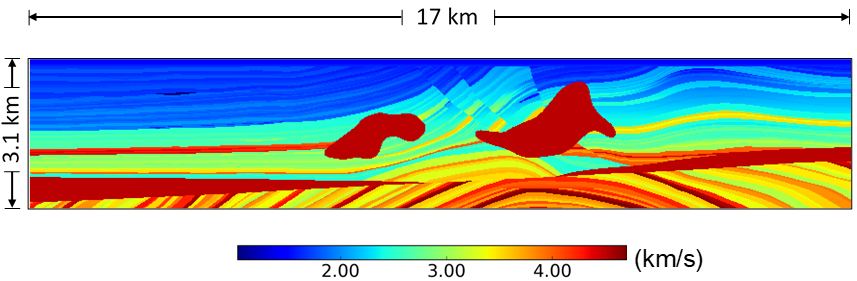
\includegraphics[scale=0.45,trim=0 0 0 0, clip]{701.png} \label{fig:701a}}
\subfloat[]{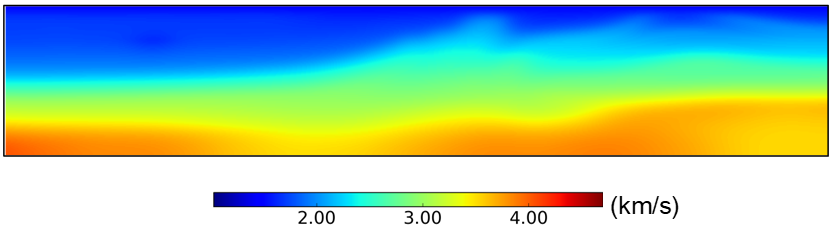
\includegraphics[scale=0.445, trim=0 0 0 -27, clip]{702.png} \label{fig:701b}}
\caption{(a) A modified Marmousi model with anomalous two salt geobodies and (b) an initial guess without presences of geobodies.}
\label{fig:701}
\end{figure}
}

\subsection{Full-waveform inversion}

Our final example is seismic waveform inversion which is also referred as full-waveform inversion (FWI).
It differs from the previous ones in three important ways.  First, in each of our previous examples the subsurface geometry consisted of a small number of shapes.  In this example, we consider a subsurface region possessing a large number of layers and two anomalous bodies. Second, we utilize full seismic waveform data which is relatively more complex than the previous geophysical data types. Third, it highlights the potential uplift from annealing strategies applied to Mumford-Shah.  

The subsurface model selected for this example is shown in Figure~\ref{fig:701a}.  It is 3.1 km deep by 17 km wide and consists of the Marmousi wave speed model with anomalies overlaid.  100 seismic sources and 500 seismic receivers are placed equidistantly on the top surface of the subsurface region from $x = 0.25$km to $16.75$km.  

Seismic measurements $p$ are computed by solving the acoustic wave equation with the free boundary conditions on the top surface and the absorbing boundary conditions along the other boundaries.  
\begin{align}
\frac{1}{\kappa}\frac{\partial^2 p}{\partial t^2} &= \nabla \cdot \left(   \frac{1}{\rho} \nabla p \right) - \nabla \cdot \frac{f}{\rho}, \label{eq:wave}\\
p=\frac{\partial p}{\partial t} &= 0 ~\text{at}~ t=0, \nonumber\\
p&=0 ~\text{on}~ \Gamma_{Free}\times[0,T], \nonumber\\
\sqrt{\frac{\rho}{\kappa}} \frac{\partial p}{\partial t}+n\cdot \nabla p &= 0 ~\text{on}~ \Gamma_{Absorbing}\times [0,T]. \nonumber
\end{align}
The density $\rho$ is set equal to 1 g/cm$^3$.  The source f corresponds to a 2 Hz low-cut Ricker wavelet with a 5 Hz peak frequency.

\sendatend{
\begin{figure}
\centering 
\subfloat[]{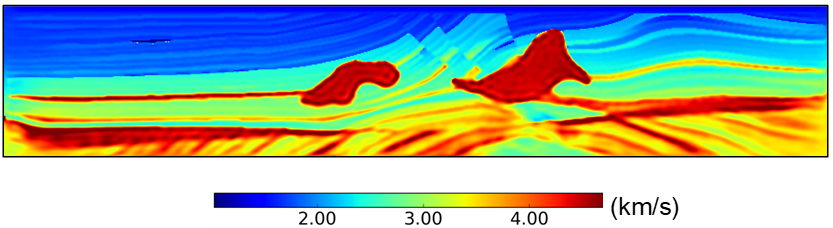
\includegraphics[scale=0.45,trim=0 0 0 0, clip]{704.png} \label{fig:704a}}
\subfloat[]{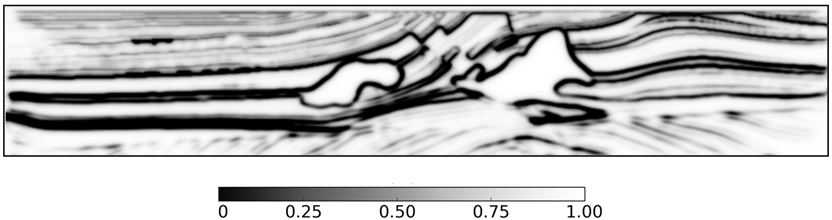
\includegraphics[scale=0.45, trim=0 0 0 0, clip]{705.png} \label{fig:704b}}
\caption{(a) The velocity model and boundary set resulting from Mumfard-Shah inversion.}
\label{fig:704}
\end{figure}
}
In this example, we focus exclusively on the Mumford-Shah inversion.  The initial guess is the wave speed profile illustrated in Figure~\ref{fig:701b} and $\phi_\epsilon=1$ (i.e. $\Gamma = \emptyset$).  The initial guess for the wave speed captures some of the large-scale trends of the Marmousi model but does not incorporate any information regarding the anomalies.  Figures~\ref{fig:704} illustrate the inverted wave speed $\kappa(x)$ and the inverted interface set $\phi_\epsilon$. The result demonstrates the ability of Mumford-Shah to determine a large number of interfaces and shapes from acoustic waveforms.

The determination of the wave speed and the boundary set require a multi-stage approach. In the first stage, equation~\ref{eq:epsilon} is minimized using $\beta=10^{-7}$.  In the second stage, the value of $\beta$ is decreased to $\beta=10^{-8}$.  In the third stage, the value of $\beta$ is decreased to $\beta =10^{-9}$.  The data misfit and model misfit versus the number of iterations are plotted in Figure~\ref{fig:706}. The branch points in Figure~\ref{fig:706} indicate where the value of $\beta$ is decreased.  Figure~\ref{fig:706} illustrates that  keeping $\beta$ fixed leads to a plateau in data and model misfit while a strategic decrease in $\beta$ results in a decrease in both data and model misfit.

\sendatend{
\begin{figure}
\centering 
\subfloat[]{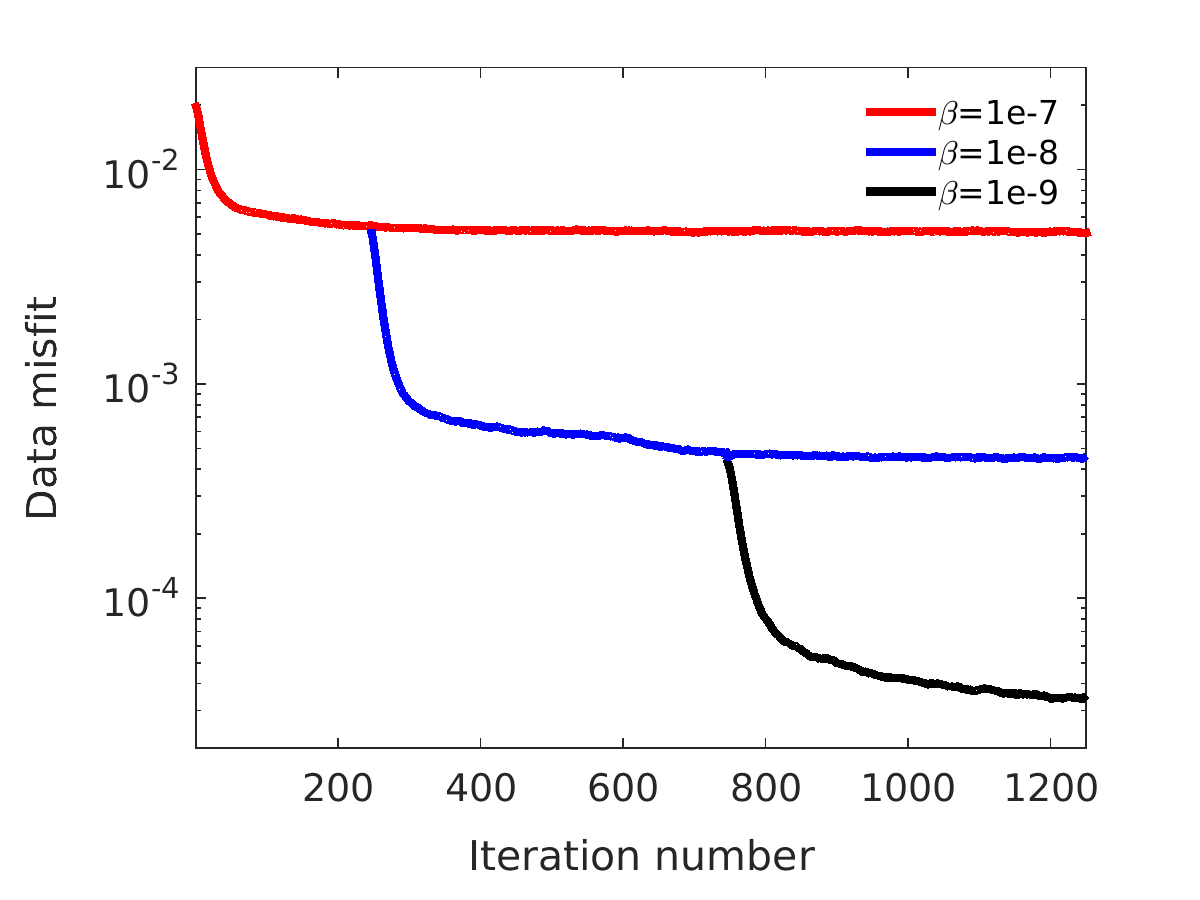
\includegraphics[scale=0.3,trim=0 0 0 0, clip]{706.png} \label{fig:706a}}
\subfloat[]{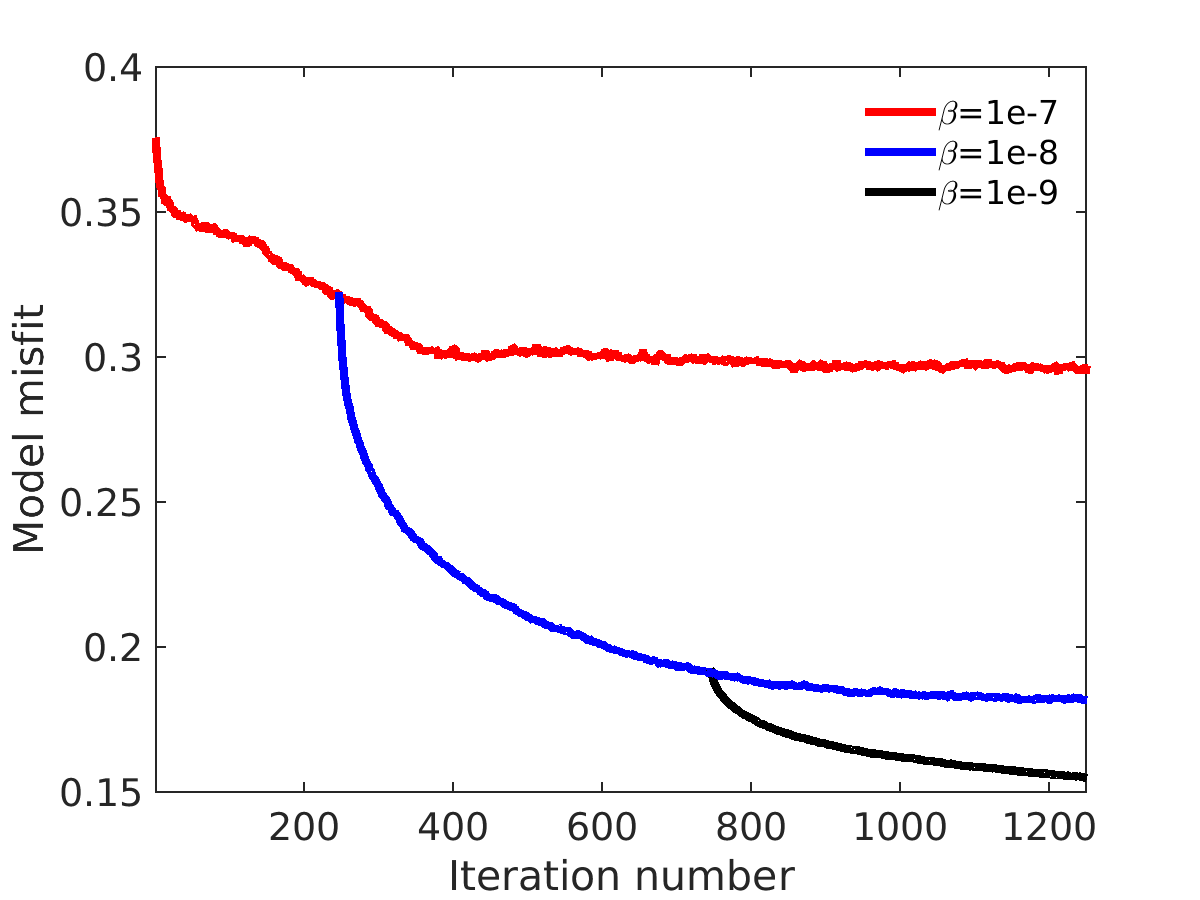
\includegraphics[scale=0.3, trim=0 0 0 0, clip]{707.png} \label{fig:706b}}
\caption{Mumford-Shah inversion: (a) data and (b) model misfits with the number of iterations.}
\label{fig:706}
\end{figure}
}

\section{Conclusion}
This paper presents two shape-based inversion algorithms to determine subsurface geophysical properties and structures in a unified manner from geophysical data. The key innovation behind these algorithms is the simultaneous inversion of interfaces and parameter values.  Jointly inverting for these ensures that the resulting parameter estimation is structurally consistent and mitigates the non-uniqueness present in cell-by-cell inversion. In addition, shape-based inversion provides a natural multi-scale framework for decomposing inverse problems that enables faster convergence to a physically reasonable solution.  

In the future, we plan to extend this framework in three directions.  First, we would like to quantify the uplift of shape-based algorithms for multi-parameter full-waveform inversion (e.g. inversion of anisotropy).  Second, we plan to investigate the performance of these algorithms for 3D geophysical inverse problems.  Third, we need to assess the robustness with respect to noise in the measurements. We also believe there are exciting applications of shape-based inversion in other scientific areas, such as medical imaging.


%\section{ACKNOWLEDGMENTS}

\newpage
\bibliographystyle{seg} 
\bibliography{main}

\newpage
\listoffigures
\newpage

\end{document}
